%
% File emnlp2020.tex
%
%% Based on the style files for ACL 2020, which were
%% Based on the style files for ACL 2018, NAACL 2018/19, which were
%% Based on the style files for ACL-2015, with some improvements
%%  taken from the NAACL-2016 style
%% Based on the style files for ACL-2014, which were, in turn,
%% based on ACL-2013, ACL-2012, ACL-2011, ACL-2010, ACL-IJCNLP-2009,
%% EACL-2009, IJCNLP-2008...
%% Based on the style files for EACL 2006 by 
%%e.agirre@ehu.es or Sergi.Balari@uab.es
%% and that of ACL 08 by Joakim Nivre and Noah Smith

\documentclass[11pt,a4paper]{article}
\usepackage[hyperref]{emnlp2020}
\usepackage{times}
\usepackage{latexsym}
\usepackage{hyperref}
\usepackage{graphicx}
\usepackage{amsmath}
\usepackage{booktabs}
\usepackage{bm}
\usepackage{multicol}
\usepackage{svg}
\usepackage{pgfplots}
\usepackage{pgfplotstable}
\usepackage{booktabs}
\usepackage{array}
\usepackage{colortbl}
% \usepackage{subcaption}
\usepackage{tikz}
\usepackage{rotating}
\pgfplotsset{compat=1.14}

\definecolor{Unbabel1}{HTML}{3843d0} % HTER model
\definecolor{Unbabel2}{HTML}{15006D} % MQM model
\definecolor{Unbabel3}{HTML}{8FA1FF}
\definecolor{Unbabel4}{HTML}{FFC466} % {\sc Bleurt}
\definecolor{Unbabel5}{HTML}{F9623E} % {\sc Bertscore}
\definecolor{Unbabel6}{HTML}{FF81A9}
\definecolor{Unbabel7}{HTML}{6ECFBD} % DARR ranker
\definecolor{ClassBlue}{HTML}{0492C2}

% \usepackage{tikz}

\renewcommand{\UrlFont}{\ttfamily\small}


% This is not strictly necessary, and may be commented out,
% but it will improve the layout of the manuscript,
% and will typically save some space.
\usepackage{microtype}

\aclfinalcopy % Uncomment this line for the final submission
\def\aclpaperid{835} %  Enter the acl Paper ID here

%\setlength\titlebox{5cm}
% You can expand the titlebox if you need extra space
% to show all the authors. Please do not make the titlebox
% smaller than 5cm (the original size); we will check this
% in the camera-ready version and ask you to change it back.

\newcommand\BibTeX{B\textsc{ib}\TeX}

\title{{\sc Comet}: A Neural Framework for MT Evaluation}

\author{Ricardo Rei \qquad Craig Stewart \qquad Ana C Farinha \qquad Alon Lavie \\ Unbabel AI\\
  {\fontsize{10}{10}\selectfont {\texttt{\{ricardo.rei, craig.stewart, catarina.farinha, alon.lavie\}@unbabel.com}}}  
}

\date{}

\begin{document}
\maketitle
\begin{abstract}
We present {\sc Comet}, a neural framework for training multilingual machine translation evaluation models which obtains new state-of-the-art levels of correlation with human judgements. Our framework leverages recent breakthroughs in cross-lingual pretrained language modeling resulting in highly multilingual and adaptable MT evaluation models that exploit information from both the source input and a target-language reference translation in order to more accurately predict MT quality. To showcase our framework, we train three models with different types of human judgements: \textit{Direct Assessments}, \textit{Human-mediated Translation Edit Rate} and \textit{Multidimensional Quality Metrics}. Our models achieve new state-of-the-art performance on the WMT 2019 Metrics shared task and demonstrate robustness to high-performing systems. %Furthermore, they show promising results towards solving the current challenges of accurate segment-level evaluation and robustness to top performing systems. 

\end{abstract}

\section{Introduction}

Historically, metrics for evaluating the quality of machine translation (MT) have relied on assessing the similarity between an MT-generated hypothesis and a human-generated reference translation in the target language.  Traditional metrics have focused on basic, lexical-level features such as counting the number of matching n-grams between the MT hypothesis and the reference translation. Metrics such as {\sc Bleu} \cite{papineni-etal-2002-bleu} and {\sc Meteor} \cite{banerjee-lavie-meteor2009} remain popular as a means of evaluating MT systems due to their light-weight and fast computation. 

Modern neural approaches to MT result in much
higher quality of translation that often deviates
from monotonic lexical transfer between languages. 
%A single reference translation might not always be sufficient to accommodate the expressiveness of such translations. 
For this reason, it has become increasingly evident that we can no longer rely on metrics such as {\sc Bleu} to provide an accurate estimate of the quality of MT \cite{barrault-etal-2019-findings}.

While an increased research interest in neural methods for training MT models and systems has resulted in a recent, dramatic improvement in MT quality, MT evaluation has fallen behind. The MT research community still relies largely on outdated metrics and no new, widely-adopted standard has emerged.  In 2019, the WMT News Translation Shared Task received a total of 153 MT system submissions \cite{barrault-etal-2019-findings}. The Metrics Shared Task of the same year saw only 24 submissions, almost half of which were entrants to the Quality Estimation Shared Task, adapted as metrics \cite{ma-etal-2019-results}. 

The findings of the above-mentioned task highlight two major challenges to MT evaluation which we seek to address herein \cite{ma-etal-2019-results}. Namely, that current metrics \textbf{struggle to accurately correlate with human judgement at segment level} and \textbf{fail to adequately differentiate the highest performing MT systems}.

%The findings of the Metrics Shared Task highlight that segment-level evaluation and strong neural MT systems are major challenges, with none of the submitted metrics achieving satisfactory levels of correlation with human judgements \cite{ma-etal-2019-results}.

In this paper, we present {\sc Comet}\footnote{\textbf{C}rosslingual \textbf{
O}ptimized \textbf{M}etric for \textbf{E}valuation of \textbf{T}ranslation.}, a PyTorch-based framework for training highly multilingual and adaptable MT evaluation models that can function as metrics. Our framework takes advantage of recent breakthroughs in cross-lingual language modeling \cite{laser2019-Artetxe, devlin-etal-2019-bert, NIPS2019_8928, conneau2019unsupervised} to generate prediction estimates of human judgments such as \textit{Direct Assessments} (DA) \cite{graham-etal-2013-continuous}, \textit{Human-mediated Translation Edit Rate} (HTER) \cite{Snover06astudy} and metrics compliant with the \textit{Multidimensional Quality Metric} framework \cite{mqm}. 

Inspired by recent work on Quality Estimation (QE) that demonstrated that it is possible to achieve high levels of correlation with human judgements even without a reference translation  \cite{fonseca-etal-2019-findings}, we propose a novel approach for incorporating the source-language input into our MT evaluation models. Traditionally only QE models have made use of the source input, whereas MT evaluation metrics rely instead on the reference translation. As in \cite{takahashi-etal-2020-automatic}, we show that using a multilingual embedding space allows us to leverage information from all three inputs and demonstrate the value added by the source as input to our MT evaluation models.

To illustrate the effectiveness and flexibility of the {\sc Comet} framework, we train three models that estimate different types of human judgements and show promising progress towards both better correlation at segment level and robustness to high-quality MT. 

%The rest of the paper is organized as follows. Section \ref{sec:literature-review} presents an overview of the related literature. Section \ref{sec:Corpora} describes the corpora used. Section \ref{sec:model} describes the different model architectures and training regimes. Section \ref{sec:experiments} describes the conducted experiments and evaluation metrics. Section \ref{sec:results} reports the corresponding results achieved. Finally, Section \ref{sec:conclusions} presents our most relevant conclusions, and pinpoints possible future directions.

We will release both the {\sc Comet} framework and the trained MT evaluation models described in this paper to the research community upon publication.

\section{Model Architectures}
\label{sec:model}
Human judgements of MT quality usually come in the form of segment-level scores, such as DA, MQM and HTER. For DA, it is common practice to convert scores into relative rankings ({\small DA}RR) when the number of annotations per segment is limited  \cite{bojar-etal-2017-results, ma-etal-2018-results, ma-etal-2019-results}. This means that, for two MT hypotheses $h_i$ and $h_j$ of the same source $s$, if the DA score assigned to $h_i$ is higher than the score assigned to $h_j$, $h_i$ is regarded as a ``better'' hypothesis.\footnote{In the WMT Metrics Shared Task, if the difference between the DA scores is not higher than 25 points, those segments are excluded from the {\scriptsize DA}RR data.} To encompass these differences, our framework supports two distinct architectures: The {\bf Estimator model} and the {\bf Translation Ranking model}. The fundamental difference between them is the training objective. While the Estimator is trained to regress directly on a quality score, the Translation Ranking model is trained to minimize the distance between a ``better'' hypothesis and both its corresponding reference and its original source. Both models are composed of a cross-lingual encoder and a pooling layer.

\subsection{Cross-lingual Encoder}
\label{ssec:encoder}
The primary building block of all the models in our framework is a pretrained, cross-lingual model such as multilingual BERT \cite{devlin-etal-2019-bert}, XLM \cite{NIPS2019_8928} or XLM-RoBERTa \cite{conneau2019unsupervised}. These models contain several transformer encoder layers that are trained to reconstruct masked tokens by uncovering the relationship between those tokens and the surrounding ones. When trained with data from multiple languages this pretrained objective has been found to be highly effective in cross-lingual tasks such as document classification and natural language inference \cite{conneau2019unsupervised}, generalizing well to unseen languages and scripts \citep{pires-etal-2019-multilingual}. For the experiments in this paper, we rely on XLM-RoBERTa (base) as our encoder model.

Given an input sequence 
$x = \left[x_0, x_1, ..., x_n\right]$, the encoder
produces an embedding
$\bm{e}_{j}^{(\ell)}$ for each token $x_j$ and each layer $\ell \in \{0,1,...,k\}$. In our framework, we apply this process to the source, MT hypothesis, and reference in order to map them into a shared feature space.

\subsection{Pooling Layer}
\label{ssec:pooling}
The embeddings generated by the last layer of the pretrained encoders are usually used for fine-tuning models to new tasks. However, \citep{tenney-etal-2019-bert} showed that different layers within the network can capture linguistic information that is relevant for different downstream tasks. In the case of MT evaluation, \citep{ZhangBERTScore} showed that different layers can achieve different levels of correlation and that utilizing only the last layer often results in inferior performance. In this work, we used the approach described in \citet{peters-etal-2018-deep} and pool information from the most important encoder layers into a single embedding for each token, $\bm{e}_{j}$, by using a layer-wise attention mechanism. This embedding is then computed as: 
\vspace{-5pt}
\begin{equation}
\label{eq:attention}
    \bm{e}_{x_j} = \mu {E}_{x_j}^\top \bm{\alpha}
\end{equation}
where $\mu$ is a trainable weight coefficient, $\bm{E}_{j} = [\bm{e}_{j}^{(0)}, \bm{e}_{j}^{(1)}, \dots\, \bm{e}_{j}^{(k)}]$ corresponds to the vector of layer embeddings for token $x_j$, and $\bm{\alpha} = \textrm{softmax} ([\alpha^{(1)}, \alpha^{(2)}, \dots, \alpha^{(k)}])$ is a vector corresponding to the layer-wise trainable weights. In order to avoid overfitting to the information contained in any single layer, we used layer dropout \cite{kondratyuk-straka-2019-75}, in which with a probability $p$ the weight $\alpha^{(i)}$ is set to $-\infty$.

Finally, as in \cite{reimers-gurevych-2019-sentence}, we apply average pooling to the resulting word embeddings to derive a sentence embedding for each segment.

\subsection{Estimator Model}
\label{ssec:estimator}

% ------------------------------------ 
% IMAGE OF OUR ESTIMATOR AND RANKING MODELS
% ------------------------------------

\begin{figure*}
    \centering
    \begin{minipage}{.48\textwidth}
        \centering
        \includegraphics[width=1.0\linewidth]{images/small_estimator.jpg}
        \caption{Estimator model architecture. The source, hypothesis and reference are independently encoded using a pretrained cross-lingual encoder. The resulting word embeddings are then passed through a pooling layer to create a sentence embedding for each segment. Finally, the resulting sentence embeddings are combined and concatenated into one single vector that is passed to a feed-forward regressor. The entire model is trained by minimizing the Mean Squared Error (MSE). }
        \label{fig:estimator}
    \end{minipage}%
    \hfill
    \begin{minipage}{.48\textwidth}
        \centering
        \vspace{25pt}
        \includegraphics[width=1.0\linewidth]{images/small_ranker.jpg}
        \caption{Translation Ranking model architecture. This architecture receives 4 segments: the source, the reference, a ``better'' hypothesis, and a ``worse'' one. These segments are independently encoded using a pretrained cross-lingual encoder and a pooling layer on top. Finally, using the triplet margin loss \cite{SchroffKP15} we optimize the resulting embedding space to minimize the distance between the ``better'' hypothesis and the ``anchors'' (source and reference).}
        \label{fig:ranking_model}
    \end{minipage}
\end{figure*}

Given a $d$-dimensional sentence embedding for the source, the hypothesis, and the reference, we adopt the approach proposed in RUSE \cite{shimanaka-etal-2018-ruse} and extract the following combined features:

\begin{itemize}
    \item Element-wise source product: $\bm{h}  \odot  \bm{s}$
    \item Element-wise reference product: $\bm{h}  \odot  \bm{r}$
    \item Absolute element-wise source difference: $|\bm{h} - \bm{s}|$
    \item Absolute element-wise reference difference: $|\bm{h} - \bm{r}|$
\end{itemize}

These combined features are then concatenated to the reference embedding $\bm{r}$ and hypothesis embedding $\bm{h}$ into a single vector $\bm{x} = [\bm{h}; \bm{r}; \bm{h}  \odot  \bm{s}; \bm{h} \odot \bm{r}; |\bm{h} - \bm{s}|; |\bm{h} - \bm{r}|]$ that serves as input to a feed-forward regressor. The strength of these features is in highlighting the differences between embeddings in the semantic feature space. 

The  model is then trained to minimize the mean squared error between the predicted scores and quality assessments (DA, HTER or MQM). Figure~\ref{fig:estimator} illustrates the proposed architecture. 

Note that we chose not to include the raw source embedding ($\bm{s}$) in our concatenated input. Early experimentation revealed that the value added by the source embedding as extra input features to our regressor was negligible at best. A variation on our HTER estimator model trained with the vector $\bm{x} = [\bm{h}; \bm{s}; \bm{r}; \bm{h}  \odot  \bm{s}; \bm{h} \odot \bm{r}; |\bm{h} - \bm{s}|; |\bm{h} - \bm{r}|]$ as input to the feed-forward only succeed in boosting segment-level performance in 8 of the 18 language pairs outlined in section \ref{sec:results} below and the average improvement in Kendall's Tau in those settings was +0.0009. As noted in \citet{zhao2020limitations}, while cross-lingual pretrained models are adaptive to multiple languages, the feature space between languages is poorly aligned. On this basis we decided in favor of excluding the source embedding on the intuition that the most important information comes from the reference embedding and reducing the feature space would allow the model to focus more on relevant information. This does not however negate the general value of the source to our model; where we include combination features such as $\bm{h} \odot \bm{s}$ and $|\bm{h} - \bm{s}|$ we do note gains in correlation as explored further in section \ref{sect:source-value} below.


% ------------------------------------
% IMAGE OF OUR ESTIMATOR MODEL
% ------------------------------------
%\begin{figure}[ht!]
%\centering
%\includegraphics[width=1.0\linewidth]{images/small_estimator.jpg}
%\caption{Estimator model architecture. The source, hypothesis and reference are independently encoded using a pretrained cross-lingual encoder. The resulting word embeddings are then passed through a pooling layer to create a sentence embedding for each segment. Finally, the resulting sentence embeddings are combined and concatenated into one single vector that is passed to a feed-forward regressor. The entire model is trained by minimizing the Mean Squared Error (MSE). }
%\label{fig:estimator}
%\end{figure}

\subsection{Translation Ranking Model}
\label{ssec:ranking}

Our Translation Ranking model (Figure \ref{fig:ranking_model}) receives as input a tuple $\chi = (s, h^{+}, h^{-}, r)$ where $h^{+}$ denotes an hypothesis that was ranked higher than another hypothesis $h^{-}$. We then pass $\chi$ through our cross-lingual encoder and pooling layer to obtain a sentence embedding for each segment in the $\chi$. Finally, using the embeddings $\{\bm{s}, \bm{h^{+}}, \bm{h^{-}}, \bm{r}\}$, we compute the triplet margin loss \cite{SchroffKP15} in relation to the source and reference:
\vspace{-10pt}
% ------------------------------------
% RANKING MODEL LOSS DEFINITION
% ------------------------------------
\begin{equation}
\label{eq:tloss}
\begin{split}
L(\chi)  &= L(\bm{s}, \bm{h^{+}}, \bm{h^{-}}) + L(\bm{r}, \bm{h^{+}}, \bm{h^{-}})
\end{split}
\end{equation}
where: \begin{equation}
\label{eq:tloss1}
\begin{split}
L(\bm{s}, \bm{h^{+}}, \bm{h^{-}}) = \\
\max\{0, d(&\bm{s}, \bm{h^{+}})\ - d(\bm{s}, \bm{h^{-}}) + \epsilon\}
\end{split}
\end{equation}

\begin{equation}
\label{eq:tloss2}
\begin{split}
L(\bm{r}, \bm{h^{+}}, \bm{h^{-}}) = \\
\max\{0, d(&\bm{r}, \bm{h^{+}})\ - d(\bm{r}, \bm{h^{-}}) + \epsilon\}
\end{split}
\end{equation}
$d(\bm{u}, \bm{v})$ denotes the euclidean distance between $\bm{u}$ and $\bm{v}$ and $\epsilon$ is a margin. Thus, during training the model optimizes the embedding space so the distance between the anchors ($\bm{s}$ and $\bm{r}$) and the ``worse'' hypothesis $\bm{h^{-}}$ is greater by at least $\epsilon$ than the distance between the anchors and ``better'' hypothesis $\bm{h^{+}}$.

During inference, the described model receives a triplet $(s, \hat{h}, r)$ with only one hypothesis. The quality score assigned to $\hat{h}$ is the harmonic mean between the distance to the source $d(\bm{s}, \bm{\hat{h}})$ and the distance to the reference $d(\bm{r}, \bm{\hat{h}})$:
\begin{equation}
\label{eq:ranking_inference}
\begin{split}
f(s, \hat{h}, r) = \frac{2 \times d(\bm{r}, \bm{\hat{h}}) \times d(\bm{s}, \bm{\hat{h}})}{d(\bm{r}, \bm{\hat{h}}) + d(\bm{s}, \bm{\hat{h}})}
\end{split}
\end{equation}

Finally, we convert the resulting distance into a similarity score bounded between 0 and 1 as follows:
\begin{equation}
\label{eq:ranking_similarity}
\begin{split}
\hat{f}(s, \hat{h}, r) = \frac{1}{1+f(s, \hat{h}, r)}
\end{split}
\end{equation}

\section{Corpora}
\label{sec:Corpora}
To demonstrate the effectiveness of our described model architectures (section \ref{sec:model}), we train three MT evaluation models where each model targets a different type of human judgment.  To train these models, we use data from three different corpora: the QT21 corpus, the {\small DA}RR from the WMT Metrics shared task (2017 to 2019) and a proprietary MQM annotated corpus. 
%Next, we will describe these corpora with all their relevant details.

\subsection{The QT21 corpus}
\label{sec:qt21}
The QT21 corpus is a publicly available\footnote{QT21 data: \url{https://lindat.mff.cuni.cz/repository/xmlui/handle/11372/LRT-2390}} dataset containing industry generated sentences from either an information technology or life sciences domains \cite{specia-etal_MTSummit:2017}. This corpus contains a total of 173K tuples with source sentence, respective human-generated reference, MT hypothesis (either from a phrase-based statistical MT or from a neural MT), and post-edited MT (PE). 
The language pairs represented in this corpus are: English to German (en-de), Latvian (en-lt) and Czech (en-cs), and German to English (de-en). 

The HTER score is obtained by computing the translation edit rate (TER) \cite{Snover06astudy} between the MT hypothesis and the corresponding PE. %Thus, HTER can then be used as a quality score that measures the effort required by a human-editor to correct a given hypothesis.
Finally, after computing the HTER for each MT, we built a training dataset $D = \{s_i, h_i, r_i, y_i\}_{n=1}^N$, where $s_i$ denotes the source text, $h_i$ denotes the MT hypothesis, $r_i$ the reference translation, and $y_i$ the HTER score for the hypothesis $h_i$. In this manner we seek to learn a regression $f(s, h, r) \rightarrow y $ that predicts the human-effort required to correct the hypothesis by looking at the source, hypothesis, and reference (but not the post-edited hypothesis).


\subsection{The WMT {\small DA}RR corpus}
\label{sec:daRR}

Since 2017, the organizers of the WMT News Translation Shared Task \cite{barrault-etal-2019-findings} have collected human judgements in the form of adequacy DAs \cite{graham-etal-2013-continuous, graham-etal-2014-machine, graham_baldwin_moffat_zobel_2017}. These DAs are then mapped into relative rankings ({\small DA}RR) \cite{ma-etal-2019-results}. The resulting data for each year (2017-19) form a dataset $D = \{s_i, h_i^+, h_i^-, r_i\}_{n=1}^N$ where $h_i^+$ denotes a ``better'' hypothesis and $h_i^-$ denotes a ``worse'' one.
Here we seek to learn a function $r(s, h, r)$ such that the score assigned to $h_i^+$ is strictly higher than the score assigned to $h_i^-$ ($r(s_i, h_i^+, r_i) > r(s_i, h_i^-, r_i)$). This data\footnote{The raw data for each year of the WMT Metrics shared task is publicly available in the results page (2019 example: \url{http://www.statmt.org/wmt19/results.html}). Note, however, that in the \texttt{README} files it is highlighted that this data is not well documented and the scripts occasionally require custom utilities that are not available.} contains a total of 24 high and low-resource language pairs such as Chinese to English (zh-en) and English to Gujarati (en-gu).

\subsection{The MQM corpus}
\label{sec:mqm}

The MQM corpus is a proprietary internal database of MT-generated translations of customer support chat messages that were annotated according to the guidelines set out in \citet{mqm_guidelines}. This data contains a total of 12K tuples, covering 12 language pairs from English to: German (en-de), Spanish (en-es), Latin-American Spanish (en-es-latam), French (en-fr), Italian (en-it), Japanese (en-ja), Dutch (en-nl), Portuguese (en-pt), Brazilian Portuguese (en-pt-br), Russian (en-ru), Swedish (en-sv), and Turkish (en-tr). Note that in this corpus English is always seen as the source language, but never as the target language. 
%This is important for some of our experiments. 
Each tuple consists of a source sentence, a human-generated reference, a MT hypothesis, and its MQM score, derived from error annotations by one (or more) trained annotators. The MQM metric referred to throughout this paper is an internal metric defined in accordance with the MQM framework \citep{mqm} (MQM). Errors are annotated under an internal typology defined under three main error types; `Style', `Fluency' and `Accuracy'. Our MQM scores range from $-\infty$ to 100 and are defined as:

% ------------------------------------
% MQM DEFINITION
% ------------------------------------
\begin{equation}
\label{eq:mqm}
\begin{split}
\text{\footnotesize MQM} = 100 - \frac{{I}_{\text{\scriptsize Minor}} + 5 \times {I}_{\text{\scriptsize Major}} 
+ 10 \times {I}_{\text{\scriptsize Crit.}}}{\text{\footnotesize Sentence Length} \times 100}
\end{split}
\end{equation}
where ${I}_{\text{\scriptsize Minor}}$ denotes the number of minor errors, ${I}_{\text{\scriptsize Major}}$ the number of major errors and ${I}_{\text{\scriptsize Crit.}}$ the number of critical errors. 

Our MQM metric takes into account the severity of the errors identified in the MT hypothesis, leading to a more fine-grained metric than HTER or DA. When used in our experiments, these values were divided by 100 and truncated at 0. As in section~\ref{sec:qt21}, we constructed a training dataset $D = \{s_i, h_i, r_i, y_i\}_{n=1}^N$, where $s_i$ denotes the source text, $h_i$ denotes the MT hypothesis, $r_i$ the reference translation, and $y_i$ the MQM score for the hypothesis $h_i$.

% ------------------------------------
% ENGLISH-TO-X RESULTS FOR WMT19
% ------------------------------------
\begin{table*}[!ht]
\centering
\caption{Kendall's Tau ($\tau$) correlations on language pairs with English as source for the WMT19 Metrics {\footnotesize DA}RR corpus. For {\sc Bertscore} we report results with the default encoder model for a complete comparison, but also with XLM-RoBERTa (base) for fairness with our models. The values reported for YiSi-1 are taken directly from the shared task paper \cite{ma-etal-2019-results}.}
\label{tab:english-to-x2019}
\begin{tabular}{lcccccccc}
\hline
\textbf{Metric}             & \textbf{en-cs} & \textbf{en-de} & \textbf{en-fi} & \textbf{en-gu} & \textbf{en-kk} & \textbf{en-lt} & \textbf{en-ru} & \textbf{en-zh} \\ \specialrule{1.5pt}{1pt}{1pt}
{\sc Bleu}                        & 0.364          & 0.248          & 0.395          & 0.463          & 0.363          & 0.333          & 0.469          & 0.235          \\
{\sc chrF}                        & 0.444          & 0.321          & 0.518          & 0.548          & 0.510          & 0.438          & 0.548          & 0.241          \\
{\sc YiSi-1}              & 0.475  &   0.351 &   0.537 & 0.551 & 0.546 & 0.470 & 0.585 & 0.355 \\
{\sc Bertscore} {\footnotesize ({default})}          & 0.500          & 0.363          & 0.527          & 0.568          & 0.540          & 0.464          & 0.585          & 0.356          \\
{\sc Bertscore} {\footnotesize ({xlmr-base})} & 0.503          & 0.369          & 0.553          & 0.584          & 0.536          & 0.514          & 0.599          & 0.317          \\ \hline
{\sc Comet-hter}              & 0.524          & 0.383          & 0.560          & 0.552          & 0.508          & 0.577          & 0.539          & 0.380          \\
{\sc Comet-mqm}               & 0.537          & 0.398          & 0.567          & 0.564          & 0.534          & 0.574          & \textbf{0.615}          & 0.378          \\
{\sc Comet-rank}                 & \textbf{0.603} & \textbf{0.427} & \textbf{0.664} & \textbf{0.611} & \textbf{0.693} & \textbf{0.665} & 0.580 & \textbf{0.449} \\ \hline
\end{tabular}
\end{table*}

\section{Experiments}
\label{sec:experiments}
We train two versions of the Estimator model described in section \ref{ssec:estimator}: one that regresses on HTER (\textbf{{\sc Comet-hter}}) trained with the QT21 corpus, and another that regresses on our proprietary implementation of MQM (\textbf{{\sc Comet-mqm}}) trained with our internal MQM corpus. For the Translation Ranking model, described in section \ref{ssec:ranking}, we train with the WMT {\small DA}RR corpus from 2017 and 2018 (\textbf{{\sc Comet-rank}}). In this section, we introduce the training setup for these models and corresponding evaluation setup.

\subsection{Training Setup}
\label{ssec:estimator_setup}
The two versions of the Estimators (\textbf{{\sc Comet-HTER/MQM}}) share the same training setup and hyper-parameters (details are included in the Appendices). For training, we load the pretrained encoder and initialize both the pooling layer and the feed-forward regressor. Whereas the layer-wise scalars $\bm{\alpha}$ from the pooling layer are initially set to zero, the weights from the feed-forward are initialized randomly. During training, we divide the model parameters into two groups: the encoder parameters, that include the encoder model and the scalars from $\bm{\alpha}$; and the regressor parameters, that include the parameters from the top feed-forward network. We apply gradual unfreezing and discriminative learning rates \cite{howard-ruder-2018-universal}, meaning that the encoder model is frozen for one epoch while the feed-forward is optimized with a learning rate of $3\mathrm{e}{-5}$. After the first epoch, the entire model is fine-tuned but the learning rate for the encoder parameters is set to $1\mathrm{e}{-5}$ in order to avoid catastrophic forgetting.

In contrast with the two Estimators, for the \textbf{{\sc Comet-rank}} model we fine-tune from the outset. Furthermore, since this model does not add any new parameters on top of XLM-RoBERTa (base) other than the layer scalars $\bm{\alpha}$, we use one single learning rate of $1\mathrm{e}{-5}$ for the entire model.

\subsection{Evaluation Setup}
\label{ssec:metrics}
We use the test data and setup of the WMT 2019 Metrics Shared Task \cite{ma-etal-2019-results} in order to compare the {\sc Comet} models with the top performing submissions of the shared task and other recent state-of-the-art metrics such as {\sc Bertscore} and {\sc Bleurt}.\footnote{To ease future research we will also provide, within our framework, detailed instructions and scripts to run other metrics such as {\sc chrF}, {\sc Bleu}, {\sc Bertscore}, and {\sc Bleurt}} The evaluation method used is the official Kendall's Tau-like formulation, $\tau$, from the WMT 2019 Metrics Shared Task \cite{ma-etal-2019-results} defined as:

\begin{equation}
    \label{eq:kendall}
    \tau = \frac{\textit{Concordant} - \textit{Discordant}}{\textit{Concordant} + \textit{Discordant}}
\end{equation}
where \textit{Concordant} is the number of times a metric assigns a higher score to the ``better'' hypothesis $h^+$ and \textit{Discordant} is the number of times a metric assigns a higher score to the ``worse'' hypothesis $h^-$ or the scores assigned to both hypotheses is the same. %Recall that, if the difference between the DA scores of two hypotheses with the same source is not higher than 25 points, those segments are excluded from the {\small DA}RR data, meaning that there are no ties in the data.

As mentioned in the findings of \cite{ma-etal-2019-results},  segment-level correlations of all submitted metrics were frustratingly low. Furthermore, all submitted metrics exhibited a dramatic lack of ability to correctly rank strong MT systems.  To evaluate whether our new MT evaluation models better address this issue, we followed the described evaluation setup used in the analysis presented in \cite{ma-etal-2019-results}, where correlation levels are examined for portions of the {\small DA}RR data that include only the top 10, 8, 6 and 4 MT systems. 

% ------------------------------------
% x-TO-ENGLISH RESULTS FOR WMT19
% ------------------------------------
\begin{table*}[!ht]
\centering
\caption{Kendall's Tau ($\tau$) correlations on language pairs with English as a target for the WMT19 Metrics {\footnotesize DA}RR corpus. As for {\sc Bertscore}, for {\sc Bleurt} we report results for two models: the base model, which is comparable in size with the encoder we used and the large model that is twice the size.}
\label{tab:x-to-english2019}
\begin{tabular}{llllllll}
\hline
\textbf{Metric}              & \textbf{de-en} & \textbf{fi-en} & \textbf{gu-en} & \textbf{kk-en} & \textbf{lt-en} & \textbf{ru-en} & \textbf{zh-en} \\ \specialrule{1.5pt}{1pt}{1pt}
{\sc Bleu}                        & 0.053          & 0.236          & 0.194          & 0.276          & 0.249          & 0.177          & 0.321          \\
{\sc chrF}                          & 0.123          & 0.292          & 0.240          & 0.323          & 0.304          & 0.115          & 0.371          \\
{\sc YiSi-1}   & 0.164     & 0.347       & 0.312       & \textbf{0.440}  & 0.376       & 0.217     & 0.426       \\
{\sc Bertscore} {\footnotesize ({default})}       & 0.190          & 0.354          & 0.292          & 0.351          & 0.381          & \textbf{0.221}          & 0.432          \\
{\sc Bertscore} {\footnotesize ({xlmr-base})} & 0.171          & 0.335          & 0.295          & 0.354          & 0.356          & 0.202          & 0.412          \\
{\sc Bleurt} {\footnotesize ({base-128})}    & 0.171          & 0.372          & 0.302          & 0.383     & 0.387          & 0.218          & 0.417          \\
{\sc Bleurt} {\footnotesize ({large-512})}            & 0.174          & 0.374          & 0.313          & 0.372          & 0.388          & 0.220          & 0.436    \\ \hline
{\sc Comet-hter}               & 0.185          & 0.333          & 0.274          & 0.297          & 0.364          & 0.163          & 0.391          \\
{\sc Comet-mqm}                & \textbf{0.207}     & 0.343          & 0.282          & 0.339          & 0.368          & 0.187          & 0.422          \\
{\sc Comet-rank}  & 0.202  & \textbf{0.399}    & \textbf{0.341}    & 0.358          & \textbf{0.407}         & 0.180 & \textbf{0.445}          \\ \hline
\end{tabular}
\end{table*}


\section{Results}
\label{sec:results}
%This section reports the results and provides an analysis of the experiments mentioned in Section \ref{sec:experiments}.

\subsection{From English into X}
\label{ssec:from-English}
Table \ref{tab:english-to-x2019} shows results for all eight language pairs with English as source.  We contrast our three {\sc Comet} models against baseline metrics such as {\sc Bleu} and {\sc chrF}, the 2019 task winning metric {\sc YiSi-1}, as well as the more recent {\sc Bertscore}.  We observe that across the board our three models trained with the {\sc Comet} framework outperform, often by significant margins, all other metrics.  Our {\small DA}RR Ranker model outperforms the two Estimators in seven out of eight language pairs. Also, even though the MQM Estimator is trained on only 12K annotated segments, it performs roughly on par with the HTER Estimator for most language-pairs, and outperforms all the other metrics in en-ru. 

\subsection{From X into English}
\label{sect:into-english}
Table \ref{tab:x-to-english2019} shows results for the seven to-English language pairs. Again, we contrast our three {\sc Comet} models against baseline metrics such as {\sc Bleu} and {\sc chrF}, the 2019 task winning metric {\sc YiSi-1}, as well as the recently published metrics {\sc Bertscore} and {\sc Bleurt}. As in Table \ref{tab:english-to-x2019} the {\small DA}RR model shows strong correlations with human judgements outperforming the recently proposed English-specific {\sc Bleurt} metric in five out of seven language pairs. Again, the MQM Estimator shows surprising strong results despite the fact that this model was trained with data that did not include English as a target. Although the encoder used in our trained models is highly multilingual, we hypothesise that this powerful ``zero-shot'' result is due to the inclusion of the source in our models.

\subsection{Language pairs not involving English}
\label{sect:no-english}
% ------------------------------------
% NOT ENGLISH RESULTS FOR WMT19
% ------------------------------------
\begin{table}[!ht]
\centering
\caption{Kendall's Tau ($\tau$) correlations on language pairs not involving English for the WMT19 Metrics {\small DA}RR corpus.}
\label{tab:not-english2019}
\begin{tabular}{llll}
\hline
\textbf{Metric}              & \textbf{de-cs} & \textbf{de-fr} & \textbf{fr-de} \\ \specialrule{1.5pt}{1pt}{1pt}
{\sc Bleu}                         & 0.222          & 0.226          & 0.173          \\
{\sc chrF}                         & 0.341          & 0.287          & 0.274          \\
{\sc YiSi-1}              & 0.376 & 0.349 & 0.310 \\
{\sc Bertscore} {\footnotesize ({default})}          & 0.358          & 0.329          & 0.300          \\
{\sc Bertscore} {\footnotesize ({xlmr-base})} & 0.386    & 0.336          & 0.309          \\ \hline
{\sc Comet-hter}               & 0.358          & 0.397          & 0.315          \\
{\sc Comet-mqm}                & 0.386          & 0.367          & 0.296          \\
{\sc Comet-rank}                  &  \textbf{0.389}          & \textbf{0.444}          & \textbf{0.331}          \\ \hline
\end{tabular}
\end{table}


All three of our {\sc Comet} models were trained on data involving English (either as a source or as a target). Nevertheless, to demonstrate that our metrics generalize well we test them on the three WMT 2019 language pairs that do not include English in either source or target. As can be seen in Table \ref{tab:not-english2019}, our results are consistent with observations in Tables \ref{tab:english-to-x2019} and \ref{tab:x-to-english2019}.  %Our three models exhibit better correlation with human judgements than previously proposed metrics.

\subsection{Robustness to High-Quality MT}
\label{sect:top-systems}

For analysis, we use the {\small DA}RR corpus from the 2019 Shared Task and evaluate on the subset of the data from the top performing MT systems for each language pair. We included language pairs for which we could retrieve data for at least ten different MT systems (i.e. all but kk-en and gu-en). We contrast against the strong recently proposed {\sc Bertscore} and {\sc Bleurt}, with {\sc Bleu} as a baseline.  Results are presented in Figure \ref{fig:Top models}. For language pairs where English is the target, our three models are either better or competitive with all others; where English is the source we note that in general our metrics exceed the performance of others. Even the MQM Estimator, trained with only 12K segments, is competitive, which highlights the power of our proposed framework.

% ------------------------------------
% PLOT FOR TOP SYSTEMS
% LEGEND:
%    red: BLEU, 
%    orange: {\sc Bertscore} (default), 
%    yellow: BLERT, 
%    turquoise: DARR Ranker, 
%    purple: MQM Estimator 
%    blue: HTER Estimator
% ------------------------------------
\begin{figure}[ht!]  
\centering 
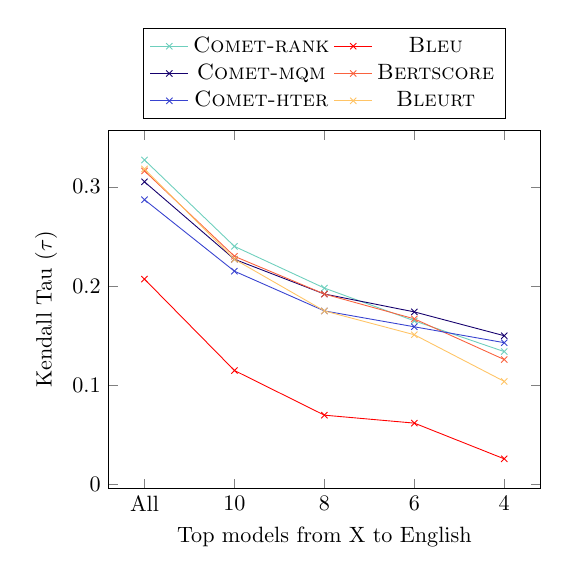
\begin{tikzpicture}[scale=0.8, transform shape]
\pgfplotsset{every axis legend/.append style={
		at={(0.5,1.03)},
		anchor=south}}
\begin{axis}[
	xlabel=Top models from X to English,
	ylabel=Kendall Tau ($\tau$),
	xticklabels={ , , All, 10 , 8, 6, 4},
	legend columns=2]
\addplot[color=Unbabel7,mark=x] coordinates {
	(1,  0.327)
	(2,  0.240)
	(3,  0.198)
	(4, 0.165)
	(5 , 0.134)
};
\addplot[color=red,mark=x] coordinates {
	(1,   0.207)
	(2,  0.115)
	(3,  0.07)
	(4, 0.062)
	(5 , 0.026)
};
\addplot[color=Unbabel2,mark=x] coordinates {
	(1,  0.305)
	(2,  0.227)
	(3,  0.192)
	(4, 0.174)
	(5 , 0.150)
};
\addplot[color=Unbabel5,mark=x] coordinates {
	(1,   0.316)
	(2,  0.230)
	(3,  0.192)
	(4, 0.167)
	(5 , 0.126)
};
\addplot[color=Unbabel1,mark=x] coordinates {
	(1,  0.287)
	(2,  0.215)
	(3,  0.175)
	(4, 0.159)
	(5 , 0.143)
};
\addplot[color=Unbabel4,mark=x] coordinates {
	(1, 0.318)
	(2,  0.227)
	(3,  0.175)
	(4, 0.151)
	(5 , 0.104])
};
\legend{{\sc Comet-rank},{\sc Bleu},{\sc Comet-mqm},{\sc Bertscore},{\sc Comet-hter}, {\sc Bleurt}}
\end{axis}
\end{tikzpicture}
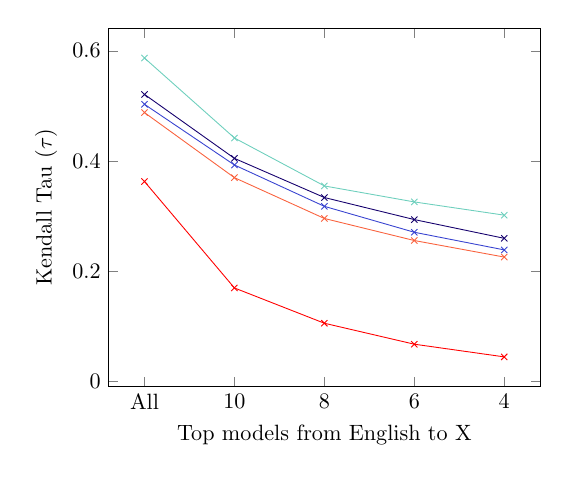
\begin{tikzpicture}[scale=0.8, transform shape]
\begin{axis}[
	xlabel=Top models from English to X,
	ylabel=Kendall Tau ($\tau$),
	xticklabels={ , , All, 10 , 8, 6, 4},
	%legend style={at={(0.5,-0.3)},anchor=north}
	]
\addplot[color=red,mark=x] coordinates {
	(1, 0.363)
	(2,  0.170)
	(3,  0.106)
	(4, 0.068)
	(5 , 0.045)
};
\addplot[color=Unbabel5,mark=x] coordinates {
	(1,  0.488)
	(2,  0.370)
	(3,  0.296)
	(4, 0.256)
	(5 , 0.226)
};
\addplot[color=Unbabel7,mark=x] coordinates {
	(1,  0.587)
	(2,  0.442)
	(3,  0.355)
	(4, 0.326)
	(5 , 0.302)
};
\addplot[color=Unbabel2,mark=x] coordinates {
	(1,  0.521)
	(2,  0.405)
	(3,  0.334)
	(4, 0.294)
	(5 , 0.260)
};
\addplot[color=Unbabel1,mark=x] coordinates {
	(1,  0.503)
	(2,  0.393)
	(3,  0.318)
	(4, 0.271)
	(5 , 0.239)
};
\end{axis}
\end{tikzpicture}
\caption{Metrics performance over all and the top (10, 8, 6, and 4) MT systems.} 
\label{fig:Top models} 
\end{figure}

\subsection{The Importance of the Source}

% ------------------------------------
% DARR Ranker REFERENCE-ONLY VS JOINT
% ------------------------------------
\begin{table*}[!ht]
\centering
\caption{Comparison between {\sc Comet-rank} (section \ref{ssec:ranking}) and a reference-only version thereof on WMT18 data. Both models were trained with WMT17 which means that the reference-only model is never exposed to English during training.} 
\label{tab:value-src}
\begin{tabular}{lllllllll}
\hline
\textbf{Metric}                                   & \textbf{en-cs} & \textbf{en-de} & \textbf{en-fi} & \textbf{en-tr}             & \textbf{cs-en} & \textbf{de-en} & \textbf{fi-en} & \textbf{tr-en} \\ \specialrule{1.5pt}{1pt}{1pt}
\multicolumn{1}{l|}{{\sc Comet-rank} \footnotesize ({ref. only})} & 0.660          & 0.764  & 0.630 & \multicolumn{1}{l|}{0.539} & 0.249 & 0.390  & 0.159  & 0.128 \\ 
\multicolumn{1}{l|}{{\sc Comet-rank}}   & 0.711 & 0.799 & 0.671 & \multicolumn{1}{l|}{0.563} & 0.356 & 0.542 & 0.278 & 0.260          \\ \hline
\multicolumn{1}{l|}{$\Delta \tau$}  & 0.051  & 0.035  & 0.041  & \multicolumn{1}{l|}{0.024} & \textbf{0.107} & \textbf{0.155} & \textbf{0.119} & \textbf{0.132} \\ \hline
\end{tabular}
\end{table*}

\label{sect:source-value}
To shed some light on the actual value and contribution of the source language input in our models' ability to learn accurate predictions, we trained two versions of our {\small DA}RR Ranker model: one that uses only the reference, and another that uses both reference and source. Both models were trained using the WMT 2017 corpus that only includes language pairs from English (en-de, en-cs, en-fi, en-tr). In other words, while English was never observed as a target language during training for both variants of the model, the training of the second variant includes English source embeddings.  We then tested these two model variants on the WMT 2018 corpus for these language pairs and for the reversed directions (with the exception of en-cs because cs-en does not exist for WMT 2018). The results in Table \ref{tab:value-src} clearly show that for the translation ranking architecture, including the source improves the overall correlation with human judgments. Furthermore, the inclusion of the source exposed the second variant of the model to English embeddings which is reflected in a higher $\Delta \tau$ for the language pairs with English as a target.

\section{Reproducibility}
\label{sec:reproducibility}
We will release both the code-base of the {\sc Comet} framework and the trained MT evaluation models described in this paper to the research community upon publication, along with the detailed scripts required in order to run all reported baselines.\footnote{These will be hosted at: \url{https://github.com/Unbabel/COMET}} All the models reported in this paper were trained on a single Tesla T4 (16GB) GPU. Moreover, our framework builds on top of PyTorch Lightning \cite{falcon2019pytorch}, a
lightweight PyTorch wrapper, that was created for maximal flexibility and reproducibility.

\section{Related Work}
\label{sec:literature-review}

Classic MT evaluation metrics are commonly characterized as \textbf{$n$-gram matching metrics} because, using hand-crafted features, they estimate MT quality by counting the number and fraction of $n$-grams that appear simultaneous in a candidate translation hypothesis and one or more human-references. Metrics such as {\sc Bleu} \cite{papineni-etal-2002-bleu}, {\sc Meteor} \cite{banerjee-lavie-meteor2009}, and {\sc chrF} \cite{popovic-2015-chrf} have been widely studied and improved \cite{koehn-etal-2007-moses, popovic-2017-chrf, denkowski-lavie-2011-meteor, guo-hu-2019-meteor}, but, by design, they usually fail to recognize and capture semantic similarity beyond the lexical level.

In recent years, word embeddings \cite{NIPS2013_5021, pennington-etal-2014-glove, peters-etal-2018-deep, devlin-etal-2019-bert} have emerged as a commonly used alternative to $n$-gram matching for capturing word semantics similarity. \textbf{Embedding-based metrics} like {\sc Meteor-Vector} \cite{servan-etal-2016-word2vec-vs}, {\sc Bleu2vec} \cite{tattar-fishel-2017-bleu2vec}, {\sc YiSi-1} \cite{lo-2019-yisi}, {\sc MoverScore} \cite{zhao-etal-2019-moverscore}, and {\sc Bertscore} \cite{ZhangBERTScore} create soft-alignments between reference and hypothesis in an embedding space and then compute a score that reflects the semantic similarity between those segments. However, human judgements such as DA and MQM, capture much more than just semantic similarity, resulting in a correlation upper-bound between human judgements and the scores produced by such metrics.

\textbf{Learnable metrics} \cite{shimanaka-etal-2018-ruse, mathur-etal-2019-putting, shimanaka2019machine} attempt to directly optimize the correlation with human judgments, and have recently shown promising results. {\sc Bleurt} \cite{Sellam&das-bleurt}, a learnable metric based on BERT \cite{devlin-etal-2019-bert}, claims state-of-the-art performance for the last 3 years of the WMT Metrics Shared task. Because {\sc Bleurt} builds on top of English-BERT \cite{devlin-etal-2019-bert}, it can only be used when English is the target language which limits its applicability. Also, to the best of our knowledge, all the previously proposed learnable metrics have focused on optimizing DA which, due to a scarcity of annotators, can prove inherently noisy \cite{ma-etal-2019-results}.

\textbf{Reference-less MT evaluation}, also known as Quality Estimation (QE), has historically often regressed on HTER for segment-level evaluation \cite{bojar-etal-2013-findings, bojar-etal-2014-findings, bojar-etal-2015-findings, bojar-etal-2016-findings, bojar-etal-2017-findings}. More recently, MQM has been used for document-level evaluation \cite{specia-etal-2018-findings, fonseca-etal-2019-findings}. By leveraging highly multilingual pretrained encoders such as multilingual BERT \cite{devlin-etal-2019-bert} and XLM \cite{NIPS2019_8928}, QE systems have been showing auspicious correlations with human judgements \cite{kepler-etal-2019-unbabels}. Concurrently, the OpenKiwi framework \cite{kepler-etal-2019-openkiwi} has made it easier for researchers to push the field forward and build stronger QE models. 

\section{Conclusions and Future Work}
\label{sec:conclusions}

In this paper we present {\sc Comet}, a novel neural framework for training MT evaluation models that can serve as automatic metrics and easily be adapted and optimized to different types of human judgements of MT quality. 

To showcase the effectiveness of our framework, we sought to address the challenges reported in the 2019 WMT Metrics Shared Task \cite{ma-etal-2019-results}. We trained three distinct models which achieve new state-of-the-art results for segment-level correlation with human judgments, and show promising ability to better differentiate high-performing systems. 

One of the challenges of leveraging the power of pretrained models is the burdensome weight of parameters and inference time. A primary avenue for future work on {\sc Comet} will look at the impact of more compact solutions such as DistilBERT \citep{sanh2019distilbert}.

Additionally, whilst we outline the potential importance of the source text above, we note that our {\sc Comet-rank} model weighs source and reference differently during inference but equally in its training loss function. Future work will investigate the optimality of this formulation and further examine the interdependence of the different inputs.

\section*{Acknowledgments}
We are grateful to Andr\'e Martins, Austin Matthews, Fabio Kepler, Daan Van Stigt, Miguel Vera, and the reviewers, for their valuable feedback and discussions. This work was supported in part by the P2020 Program through projects MAIA and Unbabel4EU, supervised by ANI under contract numbers 045909 and 042671, respectively.

\begin{thebibliography}{53}
\expandafter\ifx\csname natexlab\endcsname\relax\def\natexlab#1{#1}\fi

\bibitem[{Artetxe and Schwenk(2019)}]{laser2019-Artetxe}
Mikel Artetxe and Holger Schwenk. 2019.
\newblock \href {https://doi.org/10.1162/tacl_a_00288} {Massively multilingual
  sentence embeddings for zero-shot cross-lingual transfer and beyond}.
\newblock \emph{Transactions of the Association for Computational Linguistics},
  7:597--610.

\bibitem[{Barrault et~al.(2019)Barrault, Bojar, Costa-juss{\`a}, Federmann,
  Fishel, Graham, Haddow, Huck, Koehn, Malmasi, Monz, M{\"u}ller, Pal, Post,
  and Zampieri}]{barrault-etal-2019-findings}
Lo{\"\i}c Barrault, Ond{\v{r}}ej Bojar, Marta~R. Costa-juss{\`a}, Christian
  Federmann, Mark Fishel, Yvette Graham, Barry Haddow, Matthias Huck, Philipp
  Koehn, Shervin Malmasi, Christof Monz, Mathias M{\"u}ller, Santanu Pal, Matt
  Post, and Marcos Zampieri. 2019.
\newblock \href {https://doi.org/10.18653/v1/W19-5301} {Findings of the 2019
  conference on machine translation ({WMT}19)}.
\newblock In \emph{Proceedings of the Fourth Conference on Machine Translation
  (Volume 2: Shared Task Papers, Day 1)}, pages 1--61, Florence, Italy.
  Association for Computational Linguistics.

\bibitem[{Bojar et~al.(2013)Bojar, Buck, Callison-Burch, Federmann, Haddow,
  Koehn, Monz, Post, Soricut, and Specia}]{bojar-etal-2013-findings}
Ond{\v{r}}ej Bojar, Christian Buck, Chris Callison-Burch, Christian Federmann,
  Barry Haddow, Philipp Koehn, Christof Monz, Matt Post, Radu Soricut, and
  Lucia Specia. 2013.
\newblock \href {https://www.aclweb.org/anthology/W13-2201} {Findings of the
  2013 {W}orkshop on {S}tatistical {M}achine {T}ranslation}.
\newblock In \emph{Proceedings of the Eighth Workshop on Statistical Machine
  Translation}, pages 1--44, Sofia, Bulgaria. Association for Computational
  Linguistics.

\bibitem[{Bojar et~al.(2014)Bojar, Buck, Federmann, Haddow, Koehn, Leveling,
  Monz, Pecina, Post, Saint-Amand, Soricut, Specia, and
  Tamchyna}]{bojar-etal-2014-findings}
Ond{\v{r}}ej Bojar, Christian Buck, Christian Federmann, Barry Haddow, Philipp
  Koehn, Johannes Leveling, Christof Monz, Pavel Pecina, Matt Post, Herve
  Saint-Amand, Radu Soricut, Lucia Specia, and Ale{\v{s}} Tamchyna. 2014.
\newblock \href {https://doi.org/10.3115/v1/W14-3302} {Findings of the 2014
  workshop on statistical machine translation}.
\newblock In \emph{Proceedings of the Ninth Workshop on Statistical Machine
  Translation}, pages 12--58, Baltimore, Maryland, USA. Association for
  Computational Linguistics.

\bibitem[{Bojar et~al.(2017{\natexlab{a}})Bojar, Chatterjee, Federmann, Graham,
  Haddow, Huang, Huck, Koehn, Liu, Logacheva, Monz, Negri, Post, Rubino,
  Specia, and Turchi}]{bojar-etal-2017-findings}
Ond{\v{r}}ej Bojar, Rajen Chatterjee, Christian Federmann, Yvette Graham, Barry
  Haddow, Shujian Huang, Matthias Huck, Philipp Koehn, Qun Liu, Varvara
  Logacheva, Christof Monz, Matteo Negri, Matt Post, Raphael Rubino, Lucia
  Specia, and Marco Turchi. 2017{\natexlab{a}}.
\newblock \href {https://doi.org/10.18653/v1/W17-4717} {Findings of the 2017
  conference on machine translation ({WMT}17)}.
\newblock In \emph{Proceedings of the Second Conference on Machine
  Translation}, pages 169--214, Copenhagen, Denmark. Association for
  Computational Linguistics.

\bibitem[{Bojar et~al.(2016)Bojar, Chatterjee, Federmann, Graham, Haddow, Huck,
  Jimeno~Yepes, Koehn, Logacheva, Monz, Negri, N{\'e}v{\'e}ol, Neves, Popel,
  Post, Rubino, Scarton, Specia, Turchi, Verspoor, and
  Zampieri}]{bojar-etal-2016-findings}
Ond{\v{r}}ej Bojar, Rajen Chatterjee, Christian Federmann, Yvette Graham, Barry
  Haddow, Matthias Huck, Antonio Jimeno~Yepes, Philipp Koehn, Varvara
  Logacheva, Christof Monz, Matteo Negri, Aur{\'e}lie N{\'e}v{\'e}ol, Mariana
  Neves, Martin Popel, Matt Post, Raphael Rubino, Carolina Scarton, Lucia
  Specia, Marco Turchi, Karin Verspoor, and Marcos Zampieri. 2016.
\newblock \href {https://doi.org/10.18653/v1/W16-2301} {Findings of the 2016
  conference on machine translation}.
\newblock In \emph{Proceedings of the First Conference on Machine Translation:
  Volume 2, Shared Task Papers}, pages 131--198, Berlin, Germany. Association
  for Computational Linguistics.

\bibitem[{Bojar et~al.(2015)Bojar, Chatterjee, Federmann, Haddow, Huck, Hokamp,
  Koehn, Logacheva, Monz, Negri, Post, Scarton, Specia, and
  Turchi}]{bojar-etal-2015-findings}
Ond{\v{r}}ej Bojar, Rajen Chatterjee, Christian Federmann, Barry Haddow,
  Matthias Huck, Chris Hokamp, Philipp Koehn, Varvara Logacheva, Christof Monz,
  Matteo Negri, Matt Post, Carolina Scarton, Lucia Specia, and Marco Turchi.
  2015.
\newblock \href {https://doi.org/10.18653/v1/W15-3001} {Findings of the 2015
  workshop on statistical machine translation}.
\newblock In \emph{Proceedings of the Tenth Workshop on Statistical Machine
  Translation}, pages 1--46, Lisbon, Portugal. Association for Computational
  Linguistics.

\bibitem[{Bojar et~al.(2017{\natexlab{b}})Bojar, Graham, and
  Kamran}]{bojar-etal-2017-results}
Ond{\v{r}}ej Bojar, Yvette Graham, and Amir Kamran. 2017{\natexlab{b}}.
\newblock \href {https://doi.org/10.18653/v1/W17-4755} {Results of the {WMT}17
  metrics shared task}.
\newblock In \emph{Proceedings of the Second Conference on Machine
  Translation}, pages 489--513, Copenhagen, Denmark. Association for
  Computational Linguistics.

\bibitem[{Burchardt and Lommel(2014)}]{mqm_guidelines}
Aljoscha Burchardt and Arle Lommel. 2014.
\newblock \href {http://www.qt21.eu/downloads/MQM-usage-guidelines.pdf}
  {Practical {G}uidelines for the {U}se of {MQM} in {S}cientific {R}esearch on
  {T}ranslation quality.}
\newblock (access date: 2020-05-26).

\bibitem[{Conneau et~al.(2019)Conneau, Khandelwal, Goyal, Chaudhary, Wenzek,
  Guzm{\'a}n, Grave, Ott, Zettlemoyer, and Stoyanov}]{conneau2019unsupervised}
Alexis Conneau, Kartikay Khandelwal, Naman Goyal, Vishrav Chaudhary, Guillaume
  Wenzek, Francisco Guzm{\'a}n, Edouard Grave, Myle Ott, Luke Zettlemoyer, and
  Veselin Stoyanov. 2019.
\newblock \href {https://arxiv.org/abs/1911.02116} {Unsupervised cross-lingual
  representation learning at scale}.
\newblock \emph{arXiv preprint arXiv:1911.02116}.

\bibitem[{Conneau and Lample(2019)}]{NIPS2019_8928}
Alexis Conneau and Guillaume Lample. 2019.
\newblock \href
  {http://papers.nips.cc/paper/8928-cross-lingual-language-model-pretraining.pdf}
  {Cross-lingual language model pretraining}.
\newblock In H.~Wallach, H.~Larochelle, A.~Beygelzimer, F.~d`Alch\'{e} Buc,
  E.~Fox, and R.~Garnett, editors, \emph{Advances in Neural Information
  Processing Systems 32}, pages 7059--7069. Curran Associates, Inc.

\bibitem[{Denkowski and Lavie(2011)}]{denkowski-lavie-2011-meteor}
Michael Denkowski and Alon Lavie. 2011.
\newblock \href {https://www.aclweb.org/anthology/W11-2107} {Meteor 1.3:
  Automatic metric for reliable optimization and evaluation of machine
  translation systems}.
\newblock In \emph{Proceedings of the Sixth Workshop on Statistical Machine
  Translation}, pages 85--91, Edinburgh, Scotland. Association for
  Computational Linguistics.

\bibitem[{Devlin et~al.(2019)Devlin, Chang, Lee, and
  Toutanova}]{devlin-etal-2019-bert}
Jacob Devlin, Ming-Wei Chang, Kenton Lee, and Kristina Toutanova. 2019.
\newblock \href {https://doi.org/10.18653/v1/N19-1423} {{BERT}: Pre-training of
  deep bidirectional transformers for language understanding}.
\newblock In \emph{Proceedings of the 2019 Conference of the North {A}merican
  Chapter of the Association for Computational Linguistics: Human Language
  Technologies, Volume 1 (Long and Short Papers)}, pages 4171--4186,
  Minneapolis, Minnesota. Association for Computational Linguistics.

\bibitem[{Falcon(2019)}]{falcon2019pytorch}
WA~Falcon. 2019.
\newblock \href {https://github. com/williamFalcon/pytorch-lightning}
  {{P}y{T}orch {L}ightning: The lightweight {P}y{T}orch wrapper for
  high-performance {AI} research}.
\newblock \emph{GitHub}.

\bibitem[{Fonseca et~al.(2019)Fonseca, Yankovskaya, Martins, Fishel, and
  Federmann}]{fonseca-etal-2019-findings}
Erick Fonseca, Lisa Yankovskaya, Andr{\'e} F.~T. Martins, Mark Fishel, and
  Christian Federmann. 2019.
\newblock \href {https://doi.org/10.18653/v1/W19-5401} {Findings of the {WMT}
  2019 shared tasks on quality estimation}.
\newblock In \emph{Proceedings of the Fourth Conference on Machine Translation
  (Volume 3: Shared Task Papers, Day 2)}, pages 1--10, Florence, Italy.
  Association for Computational Linguistics.

\bibitem[{Graham et~al.(2013)Graham, Baldwin, Moffat, and
  Zobel}]{graham-etal-2013-continuous}
Yvette Graham, Timothy Baldwin, Alistair Moffat, and Justin Zobel. 2013.
\newblock \href {https://www.aclweb.org/anthology/W13-2305} {Continuous
  measurement scales in human evaluation of machine translation}.
\newblock In \emph{Proceedings of the 7th Linguistic Annotation Workshop and
  Interoperability with Discourse}, pages 33--41, Sofia, Bulgaria. Association
  for Computational Linguistics.

\bibitem[{Graham et~al.(2014)Graham, Baldwin, Moffat, and
  Zobel}]{graham-etal-2014-machine}
Yvette Graham, Timothy Baldwin, Alistair Moffat, and Justin Zobel. 2014.
\newblock \href {https://doi.org/10.3115/v1/E14-1047} {Is machine translation
  getting better over time?}
\newblock In \emph{Proceedings of the 14th Conference of the {E}uropean Chapter
  of the Association for Computational Linguistics}, pages 443--451,
  Gothenburg, Sweden. Association for Computational Linguistics.

\bibitem[{Graham et~al.(2017)Graham, Baldwin, Moffat, and
  Zobel}]{graham_baldwin_moffat_zobel_2017}
Yvette Graham, Timothy Baldwin, Alistair Moffat, and Justin Zobel. 2017.
\newblock \href {https://doi.org/10.1017/S1351324915000339} {Can machine
  translation systems be evaluated by the crowd alone}.
\newblock \emph{Natural Language Engineering}, 23(1):3–30.

\bibitem[{Guo and Hu(2019)}]{guo-hu-2019-meteor}
Yinuo Guo and Junfeng Hu. 2019.
\newblock \href {https://doi.org/10.18653/v1/W19-5357} {Meteor++ 2.0: Adopt
  syntactic level paraphrase knowledge into machine translation evaluation}.
\newblock In \emph{Proceedings of the Fourth Conference on Machine Translation
  (Volume 2: Shared Task Papers, Day 1)}, pages 501--506, Florence, Italy.
  Association for Computational Linguistics.

\bibitem[{Howard and Ruder(2018)}]{howard-ruder-2018-universal}
Jeremy Howard and Sebastian Ruder. 2018.
\newblock \href {https://doi.org/10.18653/v1/P18-1031} {Universal language
  model fine-tuning for text classification}.
\newblock In \emph{Proceedings of the 56th Annual Meeting of the Association
  for Computational Linguistics (Volume 1: Long Papers)}, pages 328--339,
  Melbourne, Australia. Association for Computational Linguistics.

\bibitem[{Kepler et~al.(2019{\natexlab{a}})Kepler, Tr{\'e}nous, Treviso, Vera,
  G{\'o}is, Farajian, Lopes, and Martins}]{kepler-etal-2019-unbabels}
Fabio Kepler, Jonay Tr{\'e}nous, Marcos Treviso, Miguel Vera, Ant{\'o}nio
  G{\'o}is, M.~Amin Farajian, Ant{\'o}nio~V. Lopes, and Andr{\'e} F.~T.
  Martins. 2019{\natexlab{a}}.
\newblock \href {https://doi.org/10.18653/v1/W19-5406} {Unbabel{'}s
  participation in the {WMT}19 translation quality estimation shared task}.
\newblock In \emph{Proceedings of the Fourth Conference on Machine Translation
  (Volume 3: Shared Task Papers, Day 2)}, pages 78--84, Florence, Italy.
  Association for Computational Linguistics.

\bibitem[{Kepler et~al.(2019{\natexlab{b}})Kepler, Tr{\'e}nous, Treviso, Vera,
  and Martins}]{kepler-etal-2019-openkiwi}
Fabio Kepler, Jonay Tr{\'e}nous, Marcos Treviso, Miguel Vera, and Andr{\'e}
  F.~T. Martins. 2019{\natexlab{b}}.
\newblock \href {https://doi.org/10.18653/v1/P19-3020} {{O}pen{K}iwi: An open
  source framework for quality estimation}.
\newblock In \emph{Proceedings of the 57th Annual Meeting of the Association
  for Computational Linguistics: System Demonstrations}, pages 117--122,
  Florence, Italy. Association for Computational Linguistics.

\bibitem[{Koehn et~al.(2007)Koehn, Hoang, Birch, Callison-Burch, Federico,
  Bertoldi, Cowan, Shen, Moran, Zens, Dyer, Bojar, Constantin, and
  Herbst}]{koehn-etal-2007-moses}
Philipp Koehn, Hieu Hoang, Alexandra Birch, Chris Callison-Burch, Marcello
  Federico, Nicola Bertoldi, Brooke Cowan, Wade Shen, Christine Moran, Richard
  Zens, Chris Dyer, Ond{\v{r}}ej Bojar, Alexandra Constantin, and Evan Herbst.
  2007.
\newblock \href {https://www.aclweb.org/anthology/P07-2045} {{M}oses: Open
  source toolkit for statistical machine translation}.
\newblock In \emph{Proceedings of the 45th Annual Meeting of the Association
  for Computational Linguistics Companion Volume Proceedings of the Demo and
  Poster Sessions}, pages 177--180, Prague, Czech Republic. Association for
  Computational Linguistics.

\bibitem[{Kondratyuk and Straka(2019)}]{kondratyuk-straka-2019-75}
Dan Kondratyuk and Milan Straka. 2019.
\newblock \href {https://doi.org/10.18653/v1/D19-1279} {75 languages, 1 model:
  Parsing universal dependencies universally}.
\newblock In \emph{Proceedings of the 2019 Conference on Empirical Methods in
  Natural Language Processing and the 9th International Joint Conference on
  Natural Language Processing (EMNLP-IJCNLP)}, pages 2779--2795, Hong Kong,
  China. Association for Computational Linguistics.

\bibitem[{Lavie and Denkowski(2009)}]{banerjee-lavie-meteor2009}
Alon Lavie and Michael Denkowski. 2009.
\newblock \href {https://doi.org/10.1007/s10590-009-9059-4} {The meteor metric
  for automatic evaluation of machine translation}.
\newblock \emph{Machine Translation}, 23:105--115.

\bibitem[{Lo(2019)}]{lo-2019-yisi}
Chi-kiu Lo. 2019.
\newblock \href {https://doi.org/10.18653/v1/W19-5358} {{Y}i{S}i - a unified
  semantic {MT} quality evaluation and estimation metric for languages with
  different levels of available resources}.
\newblock In \emph{Proceedings of the Fourth Conference on Machine Translation
  (Volume 2: Shared Task Papers, Day 1)}, pages 507--513, Florence, Italy.
  Association for Computational Linguistics.

\bibitem[{Lommel et~al.(2014)Lommel, Burchardt, and Uszkoreit}]{mqm}
Arle Lommel, Aljoscha Burchardt, and Hans Uszkoreit. 2014.
\newblock \href {https://doi.org/10.5565/rev/tradumatica.77} {Multidimensional
  quality metrics ({MQM}): A framework for declaring and describing translation
  quality metrics}.
\newblock \emph{Tradumàtica: tecnologies de la traducció}, 0:455--463.

\bibitem[{Ma et~al.(2018)Ma, Bojar, and Graham}]{ma-etal-2018-results}
Qingsong Ma, Ond{\v{r}}ej Bojar, and Yvette Graham. 2018.
\newblock \href {https://doi.org/10.18653/v1/W18-6450} {Results of the {WMT}18
  metrics shared task: Both characters and embeddings achieve good
  performance}.
\newblock In \emph{Proceedings of the Third Conference on Machine Translation:
  Shared Task Papers}, pages 671--688, Belgium, Brussels. Association for
  Computational Linguistics.

\bibitem[{Ma et~al.(2019)Ma, Wei, Bojar, and Graham}]{ma-etal-2019-results}
Qingsong Ma, Johnny Wei, Ond{\v{r}}ej Bojar, and Yvette Graham. 2019.
\newblock \href {https://doi.org/10.18653/v1/W19-5302} {Results of the {WMT}19
  metrics shared task: Segment-level and strong {MT} systems pose big
  challenges}.
\newblock In \emph{Proceedings of the Fourth Conference on Machine Translation
  (Volume 2: Shared Task Papers, Day 1)}, pages 62--90, Florence, Italy.
  Association for Computational Linguistics.

\bibitem[{Mathur et~al.(2019)Mathur, Baldwin, and
  Cohn}]{mathur-etal-2019-putting}
Nitika Mathur, Timothy Baldwin, and Trevor Cohn. 2019.
\newblock \href {https://doi.org/10.18653/v1/P19-1269} {Putting evaluation in
  context: Contextual embeddings improve machine translation evaluation}.
\newblock In \emph{Proceedings of the 57th Annual Meeting of the Association
  for Computational Linguistics}, pages 2799--2808, Florence, Italy.
  Association for Computational Linguistics.

\bibitem[{Mikolov et~al.(2013)Mikolov, Sutskever, Chen, Corrado, and
  Dean}]{NIPS2013_5021}
Tomas Mikolov, Ilya Sutskever, Kai Chen, Greg~S Corrado, and Jeff Dean. 2013.
\newblock \href
  {http://papers.nips.cc/paper/5021-distributed-representations-of-words-and-phrases-and-their-compositionality.pdf}
  {Distributed representations of words and phrases and their
  compositionality}.
\newblock In \emph{Advances in Neural Information Processing Systems 26}, pages
  3111--3119. Curran Associates, Inc.

\bibitem[{Papineni et~al.(2002)Papineni, Roukos, Ward, and
  Zhu}]{papineni-etal-2002-bleu}
Kishore Papineni, Salim Roukos, Todd Ward, and Wei-Jing Zhu. 2002.
\newblock \href {https://doi.org/10.3115/1073083.1073135} {{B}leu: a method for
  automatic evaluation of machine translation}.
\newblock In \emph{Proceedings of the 40th Annual Meeting of the Association
  for Computational Linguistics}, pages 311--318, Philadelphia, Pennsylvania,
  USA. Association for Computational Linguistics.

\bibitem[{Pennington et~al.(2014)Pennington, Socher, and
  Manning}]{pennington-etal-2014-glove}
Jeffrey Pennington, Richard Socher, and Christopher Manning. 2014.
\newblock \href {https://doi.org/10.3115/v1/D14-1162} {{G}love: Global vectors
  for word representation}.
\newblock In \emph{Proceedings of the 2014 Conference on Empirical Methods in
  Natural Language Processing ({EMNLP})}, pages 1532--1543, Doha, Qatar.
  Association for Computational Linguistics.

\bibitem[{Peters et~al.(2018)Peters, Neumann, Iyyer, Gardner, Clark, Lee, and
  Zettlemoyer}]{peters-etal-2018-deep}
Matthew Peters, Mark Neumann, Mohit Iyyer, Matt Gardner, Christopher Clark,
  Kenton Lee, and Luke Zettlemoyer. 2018.
\newblock \href {https://doi.org/10.18653/v1/N18-1202} {Deep contextualized
  word representations}.
\newblock In \emph{Proceedings of the 2018 Conference of the North {A}merican
  Chapter of the Association for Computational Linguistics: Human Language
  Technologies, Volume 1 (Long Papers)}, pages 2227--2237, New Orleans,
  Louisiana. Association for Computational Linguistics.

\bibitem[{Pires et~al.(2019)Pires, Schlinger, and
  Garrette}]{pires-etal-2019-multilingual}
Telmo Pires, Eva Schlinger, and Dan Garrette. 2019.
\newblock \href {https://doi.org/10.18653/v1/P19-1493} {How multilingual is
  multilingual {BERT}?}
\newblock In \emph{Proceedings of the 57th Annual Meeting of the Association
  for Computational Linguistics}, pages 4996--5001, Florence, Italy.
  Association for Computational Linguistics.

\bibitem[{Popovi{\'c}(2015)}]{popovic-2015-chrf}
Maja Popovi{\'c}. 2015.
\newblock \href {https://doi.org/10.18653/v1/W15-3049} {chr{F}: character
  n-gram f-score for automatic {MT} evaluation}.
\newblock In \emph{Proceedings of the Tenth Workshop on Statistical Machine
  Translation}, pages 392--395, Lisbon, Portugal. Association for Computational
  Linguistics.

\bibitem[{Popovi{\'c}(2017)}]{popovic-2017-chrf}
Maja Popovi{\'c}. 2017.
\newblock \href {https://doi.org/10.18653/v1/W17-4770} {chr{F}++: words helping
  character n-grams}.
\newblock In \emph{Proceedings of the Second Conference on Machine
  Translation}, pages 612--618, Copenhagen, Denmark. Association for
  Computational Linguistics.

\bibitem[{Reimers and Gurevych(2019)}]{reimers-gurevych-2019-sentence}
Nils Reimers and Iryna Gurevych. 2019.
\newblock \href {https://doi.org/10.18653/v1/D19-1410} {Sentence-{BERT}:
  Sentence embeddings using {S}iamese {BERT}-networks}.
\newblock In \emph{Proceedings of the 2019 Conference on Empirical Methods in
  Natural Language Processing and the 9th International Joint Conference on
  Natural Language Processing (EMNLP-IJCNLP)}, pages 3982--3992, Hong Kong,
  China. Association for Computational Linguistics.

\bibitem[{Sanh et~al.(2019)Sanh, Debut, Chaumond, and
  Wolf}]{sanh2019distilbert}
Victor Sanh, Lysandre Debut, Julien Chaumond, and Thomas Wolf. 2019.
\newblock \href {https://arxiv.org/abs/1910.01108} {Distilbert, a distilled
  version of {BERT}: smaller, faster, cheaper and lighter}.
\newblock \emph{arXiv preprint arXiv:1910.01108}.

\bibitem[{{Schroff} et~al.(2015){Schroff}, {Kalenichenko}, and
  {Philbin}}]{SchroffKP15}
F.~{Schroff}, D.~{Kalenichenko}, and J.~{Philbin}. 2015.
\newblock \href {https://ieeexplore.ieee.org/document/7298682} {Facenet: A
  unified embedding for face recognition and clustering}.
\newblock In \emph{2015 IEEE Conference on Computer Vision and Pattern
  Recognition (CVPR)}, pages 815--823.

\bibitem[{Sellam et~al.(2020)Sellam, Das, and Parikh}]{Sellam&das-bleurt}
Thibault Sellam, Dipanjan Das, and Ankur Parikh. 2020.
\newblock \href {https://doi.org/10.18653/v1/2020.acl-main.704} {{BLEURT}:
  Learning robust metrics for text generation}.
\newblock In \emph{Proceedings of the 58th Annual Meeting of the Association
  for Computational Linguistics}, pages 7881--7892, Online. Association for
  Computational Linguistics.

\bibitem[{Servan et~al.(2016)Servan, B{\'e}rard, Elloumi, Blanchon, and
  Besacier}]{servan-etal-2016-word2vec-vs}
Christophe Servan, Alexandre B{\'e}rard, Zied Elloumi, Herv{\'e} Blanchon, and
  Laurent Besacier. 2016.
\newblock \href {https://www.aclweb.org/anthology/C16-1110} {{W}ord2{V}ec vs
  {DB}nary: Augmenting {METEOR} using vector representations or lexical
  resources?}
\newblock In \emph{Proceedings of {COLING} 2016, the 26th International
  Conference on Computational Linguistics: Technical Papers}, pages 1159--1168,
  Osaka, Japan. The COLING 2016 Organizing Committee.

\bibitem[{Shimanaka et~al.(2018)Shimanaka, Kajiwara, and
  Komachi}]{shimanaka-etal-2018-ruse}
Hiroki Shimanaka, Tomoyuki Kajiwara, and Mamoru Komachi. 2018.
\newblock \href {https://doi.org/10.18653/v1/W18-6456} {{RUSE}: Regressor using
  sentence embeddings for automatic machine translation evaluation}.
\newblock In \emph{Proceedings of the Third Conference on Machine Translation:
  Shared Task Papers}, pages 751--758, Belgium, Brussels. Association for
  Computational Linguistics.

\bibitem[{Shimanaka et~al.(2019)Shimanaka, Kajiwara, and
  Komachi}]{shimanaka2019machine}
Hiroki Shimanaka, Tomoyuki Kajiwara, and Mamoru Komachi. 2019.
\newblock \href {https://arxiv.org/abs/1907.12679} {{M}achine {T}ranslation
  {E}valuation with {BERT} {R}egressor}.
\newblock \emph{arXiv preprint arXiv:1907.12679}.

\bibitem[{Snover et~al.(2006)Snover, Dorr, Schwartz, Micciulla, and
  Makhoul}]{Snover06astudy}
Matthew Snover, Bonnie Dorr, Richard Schwartz, Linnea Micciulla, and John
  Makhoul. 2006.
\newblock \href {https://www.cs.umd.edu/~snover/pub/amta06/ter_amta.pdf} {A
  study of translation edit rate with targeted human annotation}.
\newblock In \emph{In Proceedings of Association for Machine Translation in the
  Americas}, pages 223--231.

\bibitem[{Specia et~al.(2018)Specia, Blain, Logacheva, Astudillo, and
  Martins}]{specia-etal-2018-findings}
Lucia Specia, Fr{\'e}d{\'e}ric Blain, Varvara Logacheva, Ram{\'o}n Astudillo,
  and Andr{\'e} F.~T. Martins. 2018.
\newblock \href {https://doi.org/10.18653/v1/W18-6451} {Findings of the {WMT}
  2018 shared task on quality estimation}.
\newblock In \emph{Proceedings of the Third Conference on Machine Translation:
  Shared Task Papers}, pages 689--709, Belgium, Brussels. Association for
  Computational Linguistics.

\bibitem[{Specia et~al.(2017)Specia, Harris, Blain, Burchardt, Macketanz,
  Skadina, Negri, , and Turchi}]{specia-etal_MTSummit:2017}
Lucia Specia, Kim Harris, Fr\'ed\'eric Blain, Aljoscha Burchardt, Viviven
  Macketanz, Inguna Skadina, Matteo Negri, , and Marco Turchi. 2017.
\newblock \href {https://www.dfki.de/lt/publication_show.php?id=9490}
  {Translation quality and productivity: A study on rich morphology languages}.
\newblock In \emph{Machine Translation Summit XVI}, pages 55--71, Nagoya,
  Japan.

\bibitem[{Takahashi et~al.(2020)Takahashi, Sudoh, and
  Nakamura}]{takahashi-etal-2020-automatic}
Kosuke Takahashi, Katsuhito Sudoh, and Satoshi Nakamura. 2020.
\newblock \href {https://doi.org/10.18653/v1/2020.acl-main.327} {Automatic
  machine translation evaluation using source language inputs and cross-lingual
  language model}.
\newblock In \emph{Proceedings of the 58th Annual Meeting of the Association
  for Computational Linguistics}, pages 3553--3558, Online. Association for
  Computational Linguistics.

\bibitem[{T{\"a}ttar and Fishel(2017)}]{tattar-fishel-2017-bleu2vec}
Andre T{\"a}ttar and Mark Fishel. 2017.
\newblock \href {https://doi.org/10.18653/v1/W17-4771} {bleu2vec: the painfully
  familiar metric on continuous vector space steroids}.
\newblock In \emph{Proceedings of the Second Conference on Machine
  Translation}, pages 619--622, Copenhagen, Denmark. Association for
  Computational Linguistics.

\bibitem[{Tenney et~al.(2019)Tenney, Das, and Pavlick}]{tenney-etal-2019-bert}
Ian Tenney, Dipanjan Das, and Ellie Pavlick. 2019.
\newblock \href {https://doi.org/10.18653/v1/P19-1452} {{BERT} rediscovers the
  classical {NLP} pipeline}.
\newblock In \emph{Proceedings of the 57th Annual Meeting of the Association
  for Computational Linguistics}, pages 4593--4601, Florence, Italy.
  Association for Computational Linguistics.

\bibitem[{Zhang et~al.(2020)Zhang, Kishore, Wu, Weinberger, and
  Artzi}]{ZhangBERTScore}
Tianyi Zhang, Varsha Kishore, Felix Wu, Kilian~Q. Weinberger, and Yoav Artzi.
  2020.
\newblock \href {https://openreview.net/forum?id=SkeHuCVFDr} {Bertscore:
  Evaluating text generation with bert}.
\newblock In \emph{International Conference on Learning Representations}.

\bibitem[{Zhao et~al.(2020)Zhao, Glava{\v{s}}, Peyrard, Gao, West, and
  Eger}]{zhao2020limitations}
Wei Zhao, Goran Glava{\v{s}}, Maxime Peyrard, Yang Gao, Robert West, and
  Steffen Eger. 2020.
\newblock \href {https://doi.org/10.18653/v1/2020.acl-main.151} {On the
  limitations of cross-lingual encoders as exposed by reference-free machine
  translation evaluation}.
\newblock In \emph{Proceedings of the 58th Annual Meeting of the Association
  for Computational Linguistics}, pages 1656--1671, Online. Association for
  Computational Linguistics.

\bibitem[{Zhao et~al.(2019)Zhao, Peyrard, Liu, Gao, Meyer, and
  Eger}]{zhao-etal-2019-moverscore}
Wei Zhao, Maxime Peyrard, Fei Liu, Yang Gao, Christian~M. Meyer, and Steffen
  Eger. 2019.
\newblock \href {https://doi.org/10.18653/v1/D19-1053} {{M}over{S}core: Text
  generation evaluating with contextualized embeddings and earth mover
  distance}.
\newblock In \emph{Proceedings of the 2019 Conference on Empirical Methods in
  Natural Language Processing and the 9th International Joint Conference on
  Natural Language Processing (EMNLP-IJCNLP)}, pages 563--578, Hong Kong,
  China. Association for Computational Linguistics.

\end{thebibliography}

\bibliographystyle{acl_natbib}

\clearpage
\appendix

\section{Appendices}

\begin{table*}[!ht]
\centering
\caption{Hyper-parameters used in our {\sc Comet} framework to train the presented models.} 
\label{tab:hyperparameters}
\begin{tabular}{lcc}
\hline
\textbf{Hyper-parameter}       & \multicolumn{1}{l}{\textbf{{\sc Comet}(Est-HTER/MQM)}} & \multicolumn{1}{l}{\textbf{{\sc Comet-rank}}} \\ \specialrule{1.5pt}{1pt}{1pt}
Encoder Model             & XLM-RoBERTa (base)                              & XLM-RoBERTa (base)                       \\
Optimizer                 & Adam (default parameters)                       & Adam (default parameters)                \\
nº frozen epochs          & 1                                               & 0                                        \\
Learning rate              & 3e-05 and 1e-05                                 & 1e-05                                    \\
Batch size                & 16                                              & 16                                       \\
Loss function             & MSE                                             & Triplet Margin ($\epsilon = 1.0$)               \\
Layer-wise dropout        & 0.1                                             & 0.1                                      \\
FP precision              & 32                                              & 32      
\\
Feed-Forward hidden units & 2304,1152                                       & --                                       \\
Feed-Forward activations  & Tanh                                            & --                                       \\
Feed-Forward dropout      & 0.1                                             & --                                       \\ \hline
\end{tabular}
\end{table*}

\label{sec:appendix}
In Table \ref{tab:hyperparameters} we list the hyper-parameters used to train our models. Before initializing these models a random seed  was set to 3 in all libraries that perform ``random'' operations (\texttt{torch}, \texttt{numpy}, \texttt{random} and \texttt{cuda}).

\begin{table*}[!ht]
\centering
\caption{Statistics for the QT21 corpus.} 
\begin{tabular}{lllll}
\hline
                      & \textbf{en-de} & \textbf{en-cs} & \textbf{en-lv} & \textbf{de-en} \\ \specialrule{1.5pt}{1pt}{1pt}
\multicolumn{1}{l|}{\textbf{Total tuples}}   & 54000 & 42000 & 35474 & 41998 \\
\multicolumn{1}{l|}{\textbf{Avg. tokens} (reference)} & 17.80 & 15.56 & 16.42 & 17.71 \\
\multicolumn{1}{l|}{\textbf{Avg. tokens} (source)} & 16.70 & 17.37 & 18.39 & 17.18 \\
\multicolumn{1}{l|}{\textbf{Avg. tokens} (MT)}  & 17.65 & 15.64 & 16.42 & 17.78 \\
\hline
\end{tabular}
\end{table*}

%table WMT2017
\begin{table*}[]
\centering
\caption{Statistics for the WMT 2017 {\footnotesize DA}RR corpus.} 
\begin{tabular}{llllll}
\hline
 & \textbf{en-cs} & \textbf{en-de} & \textbf{en-fi} & \textbf{en-lv} & \textbf{en-tr} \\ \specialrule{1.5pt}{1pt}{1pt}
\multicolumn{1}{l|}{\textbf{Total tuples}} & 32810 & 6454  & 3270  & 3456  & 247   \\
\multicolumn{1}{l|}{\textbf{Avg. tokens} (reference)} & 19.70 & 22.15 & 15.59 & 21.42 & 17.57 \\
\multicolumn{1}{l|}{\textbf{Avg. tokens} (source)} & 22.37 & 23.41 & 21.73 & 26.08 & 22.51 \\
\multicolumn{1}{l|}{\textbf{Avg. tokens} (MT)}  & 19.45 & 22.58 & 16.06 & 22.18 & 17.25 \\
\hline
\end{tabular}
\end{table*}

%table WMT2019 into-English
\begin{sidewaystable}
\centering
\caption{Statistics for the WMT 2019 {\footnotesize DA}RR into-English language pairs.} 
\begin{tabular}{llllllll}
\hline
 & \textbf{de-en} & \textbf{fi-en} & \textbf{gu-en} & \textbf{kk-en} & \textbf{lt-en} & \textbf{ru-en} & \textbf{zh-en} \\ \specialrule{1.5pt}{1pt}{1pt}
\multicolumn{1}{l|}{\textbf{Total tuples}}   & 85365 & 32179 & 20110 & 9728  & 21862 & 39852 & 31070 \\
\multicolumn{1}{l|}{\textbf{Avg. tokens} (reference)} & 20.29 & 18.55 & 17.64 & 20.36 & 26.55 & 21.74 & 42.89  \\
\multicolumn{1}{l|}{\textbf{Avg. tokens} (source)}   & 18.44 & 12.49 & 21.92 & 16.32 & 20.32 & 18.00 & 7.57   \\
\multicolumn{1}{l|}{\textbf{Avg. tokens} (MT)} & 20.22 & 17.76 & 17.02 & 19.68 & 25.25 & 21.80 & 39.70  \\
\hline
\end{tabular}
\end{sidewaystable}

%table WMT2019 from-English + no-English
\begin{sidewaystable}
\centering
\caption{Statistics for the WMT 2019 {\footnotesize DA}RR from-English and no-English language pairs.}
\begin{tabular}{llllllllllll}
\hline
 & \textbf{en-cs} & \textbf{en-de} &  \textbf{en-fi} & \textbf{en-gu} & \textbf{en-kk} & \textbf{en-lt} & \textbf{en-ru} & \textbf{en-zh} & \textbf{fr-de} & \textbf{de-cs} & \textbf{de-fr} \\ \specialrule{1.5pt}{1pt}{1pt}
\multicolumn{1}{l|}{\textbf{Total tuples}}   & 27178 & 99840 &  31820 & 11355 & 18172 & 17401 & 24334 & 18658 & 1369  & 23194 & 4862  \\
\multicolumn{1}{l|}{\textbf{Avg. tokens} (reference)} & 22.92 & 25.65 &  20.12 & 33.32 & 18.89 & 21.00 & 24.79 & 9.25  & 22.68 & 22.27 & 27.32 \\
\multicolumn{1}{l|}{\textbf{Avg. tokens} (source)}    & 24.98 & 24.97 &  25.23 & 24.32 & 23.78 & 24.46 & 24.45 & 24.39 & 28.60 & 25.22 & 21.36 \\
\multicolumn{1}{l|}{\textbf{Avg. tokens} (MT)}        & 22.60 & 24.98 &  19.69 & 32.97 & 19.92 & 20.97 & 23.37 & 6.83  & 23.36 & 21.89 & 25.68 \\
\hline
\end{tabular}
\end{sidewaystable}

\begin{sidewaystable}
\centering
\caption{MQM corpus (section \ref{sec:mqm}) statistics.} 
\begin{tabular}{lllllllllllll}
\hline
    & \textbf{en-nl} & \textbf{en-sv} & \textbf{en-ja} & \textbf{en-de} & \textbf{en-ru} & \textbf{en-es} & \textbf{en-fr} & \textbf{en-it} & \textbf{en-pt-br} & \textbf{en-tr} & \textbf{en-pt} & \textbf{en-es-latam} \\ \specialrule{1.5pt}{1pt}{1pt}
\multicolumn{1}{l|}{\textbf{Total tuples}}    & 2447  & 970   & 1590  & 2756  & 1043  & 259   & 1474  & 812   & 504      & 370   & 91    & 6           \\
\multicolumn{1}{l|}{\textbf{Avg. tokens} (reference)} & 14.10 & 14.24 & 20.32 & 13.78 & 13.37 & 10.90 & 13.75 & 13.61 & 12.48    & 7.95  & 12.18 & 10.33       \\
\multicolumn{1}{l|}{\textbf{Avg. tokens} (source)} & 14.23 & 15.31 & 13.69 & 13.76 & 13.94 & 11.23 & 12.85 & 14.22 & 12.46    & 10.36 & 13.45 & 12.33       \\
\multicolumn{1}{l|}{\textbf{Avg. tokens} (MT)}  & 13.66 & 13.91 & 17.84 & 13.41 & 13.19 & 10.88 & 13.59 & 13.02 & 12.19    & 7.99  & 12.21 & 10.17 \\
\hline
\end{tabular}
\end{sidewaystable}

\begin{sidewaystable}[]
\centering
\caption{Statistics for the WMT 2018 {\footnotesize DA}RR language pairs.}
\begin{tabular}{lllllllllllllll}
\hline
                      & \textbf{zh-en} & \textbf{en-zh} & \textbf{cs-en} & \textbf{fi-en} & \textbf{ru-en} & \textbf{tr-en} & \textbf{de-en} & \textbf{en-cs} & \textbf{en-de} & \textbf{en-et} & \textbf{en-fi} & \textbf{en-ru} & \textbf{en-tr} & \textbf{et-en} \\ \specialrule{1.5pt}{1pt}{1pt}
\multicolumn{1}{l|}{\textbf{Total tuples}}  & 33357 & 28602 & 5110  & 15648 & 10404 & 8525  & 77811 & 5413  & 19711 & 32202 & 9809  & 22181 & 1358  & 56721 \\
\multicolumn{1}{l|}{\textbf{Avg. tokens} (reference)} & 28.86 & 24.04 & 21.98 & 21.13 & 24.97 & 23.25 & 23.29 & 19.50 & 23.54 & 18.21 & 16.32 & 21.81 & 20.15 & 23.40 \\
\multicolumn{1}{l|}{\textbf{Avg. tokens} (source)} & 23.86 & 28.27 & 18.67 & 15.03 & 21.37 & 18.80 & 21.95 & 22.67 & 24.82 & 23.47 & 22.82 & 25.24 & 24.37 & 18.15 \\
\multicolumn{1}{l|}{\textbf{Avg. tokens} (MT)}  & 27.45 & 14.94 & 21.79 & 20.46 & 25.25 & 22.80 & 22.64 & 19.73 & 23.74 & 18.37 & 17.15 & 21.86 & 19.61 & 23.52 \\
\hline
\end{tabular}
\end{sidewaystable}


\newcommand{\hwplotA}{\raisebox{2pt}{\tikz{\draw[red,solid,line width=0.9pt](0,0) -- (5mm,0);}}}
\newcommand{\hwplotB}{\raisebox{2pt}{\tikz{\draw[Unbabel1,solid,line width=1.2pt](0,0) -- (5mm,0);}}}
\newcommand{\hwplotC}{\raisebox{2pt}{\tikz{\draw[Unbabel2,solid,line width=1.2pt](0,0) -- (5mm,0);}}}
\newcommand{\hwplotD}{\raisebox{2pt}{\tikz{\draw[Unbabel5,solid,line width=1.2pt](0,0) -- (5mm,0);}}}
\newcommand{\hwplotE}{\raisebox{2pt}{\tikz{\draw[Unbabel7,solid,line width=1.2pt](0,0) -- (5mm,0);}}}
\newcommand{\hwplotF}{\raisebox{2pt}{\tikz{\draw[Unbabel4,solid,line width=1.2pt](0,0) -- (5mm,0);}}}


\pgfplotsset{
	small,
}
\begin{table*}
\centering
	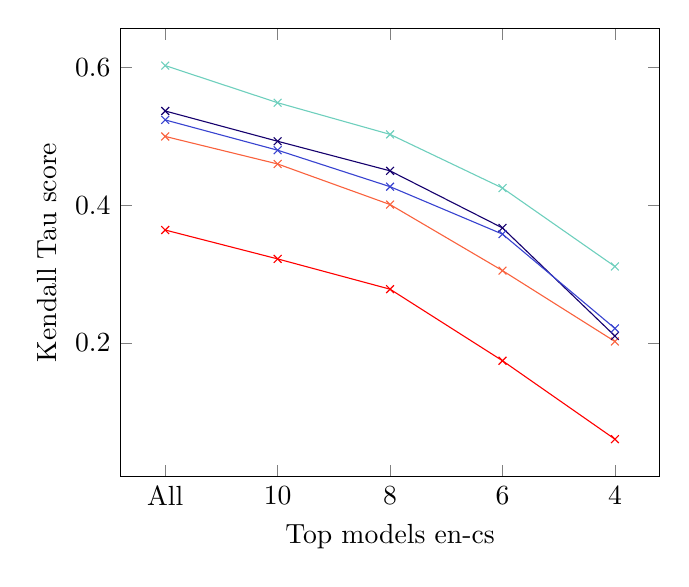
\begin{tikzpicture}
		\begin{axis}[
            xlabel=Top models en-cs, 
            ylabel=Kendall Tau score,
            xticklabels={ , , All, 10 , 8, 6, 4}
        ]
        \addplot[color=red,mark=x] coordinates {
        	(1, 0.364)
        	(2,  0.322)
        	(3,  0.278)
        	(4, 0.174)
        	(5 , 0.060)
        };
        
        \addplot[color=Unbabel5,mark=x] coordinates {
        	(1,  0.500)
        	(2,  0.460)
        	(3, 0.401)
        	(4, 0.305)
        	(5 , 0.202)
        };
        
        \addplot[color=Unbabel7,mark=x] coordinates {
        	(1,  0.603)
        	(2,  0.549)
        	(3,  0.503)
        	(4, 0.425)
        	(5 , 0.311)
        };
        
        \addplot[color=Unbabel2,mark=x] coordinates {
        	(1,  0.537)
        	(2,  0.493)
        	(3,  0.450)
        	(4, 0.367)
        	(5 , 0.210)
        };
        
        \addplot[color=Unbabel1,mark=x] coordinates {
        	(1,  0.524)
        	(2,  0.480)
        	(3,  0.427)
        	(4, 0.358)
        	(5 ,0.221)
        };
        \end{axis}
	\end{tikzpicture}
	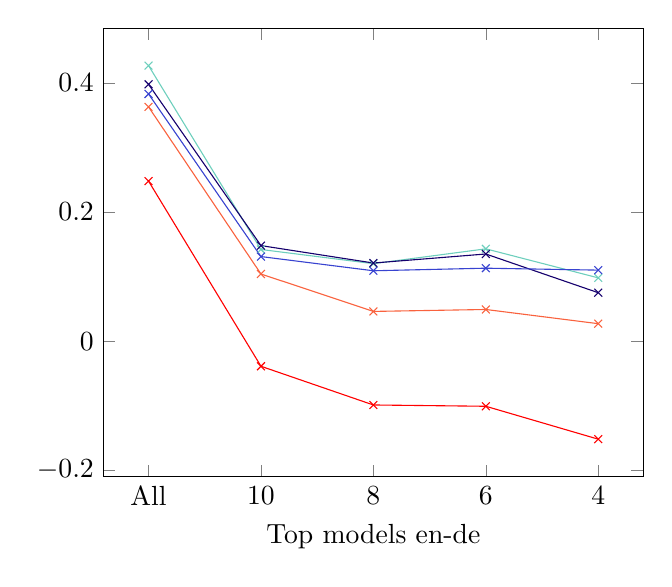
\begin{tikzpicture}
	\begin{axis}[
                    xlabel=Top models en-de, 
                    %ylabel=Kendall Tau score,
                    xticklabels={ , , All, 10 , 8, 6, 4}
                ]
        
        \addplot[color=red,mark=x] coordinates {
        	(1, 0.248)
        	(2,  -0.039)
        	(3,  -0.099)
        	(4, -0.101)
        	(5 ,-0.152)
        };
        
        \addplot[color=Unbabel5,mark=x] coordinates {
        	(1,  0.363)
        	(2, 0.104)
        	(3, 0.046)
        	(4, 0.049)
        	(5 , 0.027)
        };
        
        \addplot[color=Unbabel7,mark=x] coordinates {
        	(1,  0.427)
        	(2,  0.142)
        	(3,  0.120)
        	(4, 0.143)
        	(5 , 0.098)
        };
        
        \addplot[color=Unbabel2,mark=x] coordinates {
        	(1,  0.398)
        	(2,  0.148)
        	(3,  0.121)
        	(4, 0.135)
        	(5 , 0.075)
        };
        
        \addplot[color=Unbabel1,mark=x] coordinates {
        	(1,  0.383)
        	(2,  0.131)
        	(3,  0.109)
        	(4, 0.113)
        	(5 ,0.110)
        };
        
        \end{axis}
	\end{tikzpicture}
	\\
	%
	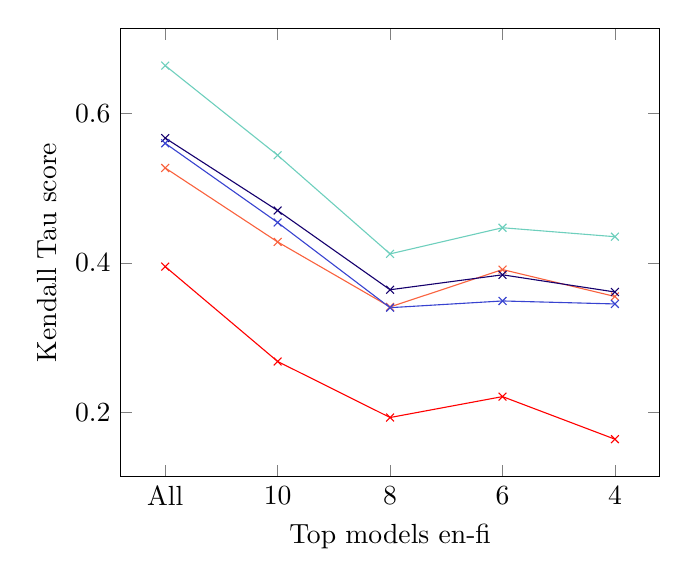
\begin{tikzpicture}
    	\begin{axis}[
                    xlabel=Top models en-fi, 
                    ylabel=Kendall Tau score,
                    xticklabels={ , , All, 10 , 8, 6, 4}
                ]
        
        \addplot[color=red,mark=x] coordinates {
        	(1, 0.395)
        	(2,  0.268)
        	(3,  0.193)
        	(4, 0.221)
        	(5 ,0.164)
        };
        
        \addplot[color=Unbabel5,mark=x] coordinates {
        	(1,  0.527)
        	(2, 0.428)
        	(3, 0.341)
        	(4, 0.391)
        	(5 , 0.355)
        };
        
        \addplot[color=Unbabel7,mark=x] coordinates {
        	(1,  0.664)
        	(2,  0.544)
        	(3,  0.412)
        	(4, 0.447)
        	(5 , 0.435)
        };
        
        \addplot[color=Unbabel2,mark=x] coordinates {
        	(1,  0.567)
        	(2,  0.470)
        	(3,  0.364)
        	(4, 0.384)
        	(5 , 0.361)
        };
        
        \addplot[color=Unbabel1,mark=x] coordinates {
        	(1,  0.560)
        	(2,  0.454)
        	(3,  0.340)
        	(4, 0.349)
        	(5 ,0.345)
        };
        
        \end{axis}
	\end{tikzpicture}%
	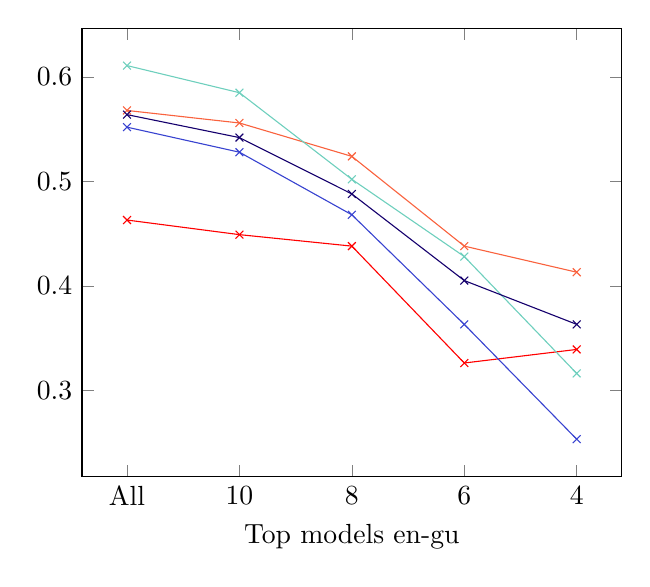
\begin{tikzpicture}
    	\begin{axis}[
                    xlabel=Top models en-gu, 
                    xticklabels={ , , All, 10 , 8, 6, 4}
                ]
        	
        \addplot[color=red,mark=x] coordinates {
        	(1, 0.463)
        	(2,  0.449)
        	(3,  0.438)
        	(4, 0.326)
        	(5 ,0.339)
        };
        
        \addplot[color=Unbabel5,mark=x] coordinates {
        	(1,  0.568)
        	(2, 0.556)
        	(3, 0.524)
        	(4, 0.438)
        	(5 , 0.413)
        };
        
        \addplot[color=Unbabel7,mark=x] coordinates {
        	(1,  0.611)
        	(2,  0.585)
        	(3,  0.502)
        	(4, 0.428)
        	(5 , 0.316)
        };
        
        \addplot[color=Unbabel2,mark=x] coordinates {
        	(1,  0.564)
        	(2,  0.542)
        	(3,  0.488)
        	(4, 00.405)
        	(5 , 0.363)
        };
        
        \addplot[color=Unbabel1,mark=x] coordinates {
        	(1,  0.552)
        	(2,  0.528)
        	(3,  0.468)
        	(4, 0.363)
        	(5 ,0.253)
        };
        \end{axis}
	\end{tikzpicture}%
	\\
	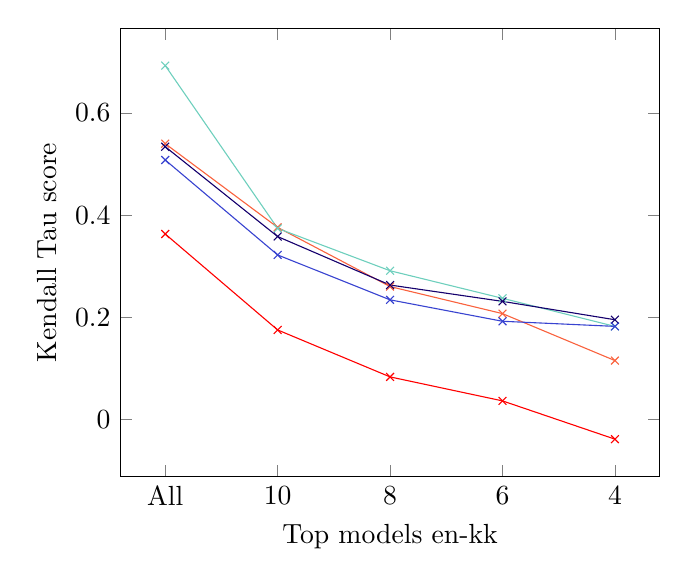
\begin{tikzpicture}
	    \begin{axis}[
            xlabel=Top models en-kk, 
            ylabel=Kendall Tau score,
            xticklabels={ , , All, 10 , 8, 6, 4}
        ]
        
        \addplot[color=red,mark=x] coordinates {
        	(1, 0.363)
        	(2,  0.175)
        	(3,  0.083)
        	(4, 0.036)
        	(5 ,-0.039)
        };
        
        \addplot[color=Unbabel5,mark=x] coordinates {
        	(1,  0.540)
        	(2, 0.376)
        	(3, 0.260)
        	(4, 0.207)
        	(5 , 0.115)
        };
        
        \addplot[color=Unbabel7,mark=x] coordinates {
        	(1,  0.693)
        	(2,  0.374)
        	(3,  0.291)
        	(4, 0.237)
        	(5 , 0.182)
        };
        
        \addplot[color=Unbabel2,mark=x] coordinates {
        	(1,  0.534)
        	(2,  0.358)
        	(3,  0.263)
        	(4, 0.231)
        	(5 , 0.195)
        };
        
        \addplot[color=Unbabel1,mark=x] coordinates {
        	(1,  0.508)
        	(2,  0.322)
        	(3,  0.234)
        	(4, 0.192)
        	(5 ,0.182)
        };
        \end{axis}  
	\end{tikzpicture}
	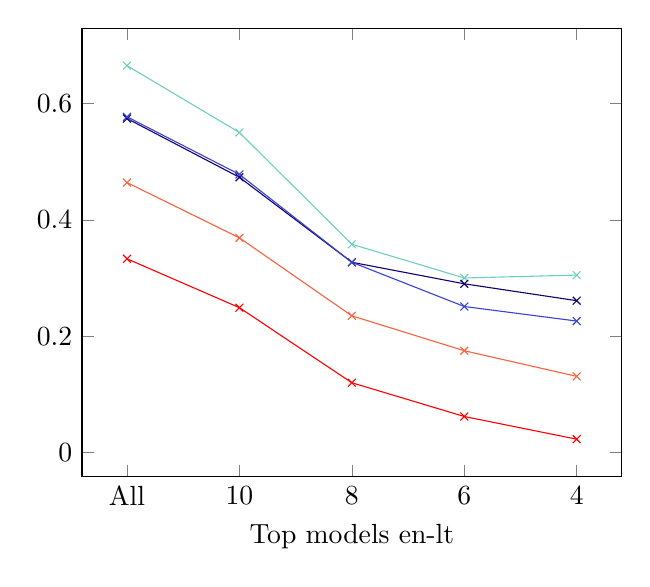
\begin{tikzpicture}
	    \begin{axis}[
            xlabel=Top models en-lt, 
            xticklabels={ , , All, 10 , 8, 6, 4}
        ]
        
        \addplot[color=red,mark=x] coordinates {
        	(1, 0.333)
        	(2,  0.249)
        	(3,  0.12)
        	(4, 0.062)
        	(5 ,0.023)
        };
        
        \addplot[color=Unbabel5,mark=x] coordinates {
        	(1,  0.464)
        	(2, 0.369)
        	(3, 0.235)
        	(4, 0.175)
        	(5 , 0.131)
        };
        
        \addplot[color=Unbabel7,mark=x] coordinates {
        	(1,  0.665)
        	(2,  0.550)
        	(3,  0.358)
        	(4, 0.300)
        	(5 , 0.305)
        };
        
        \addplot[color=Unbabel2,mark=x] coordinates {
        	(1,  0.574)
        	(2,  0.473)
        	(3,  0.327)
        	(4, 0.290)
        	(5 , 0.261)
        };
        
        \addplot[color=Unbabel1,mark=x] coordinates {
        	(1,  0.577)
        	(2,  0.478)
        	(3,  0.327)
        	(4, 0.251)
        	(5 ,0.226)
        };
        \end{axis}
        \end{tikzpicture}
    \\
    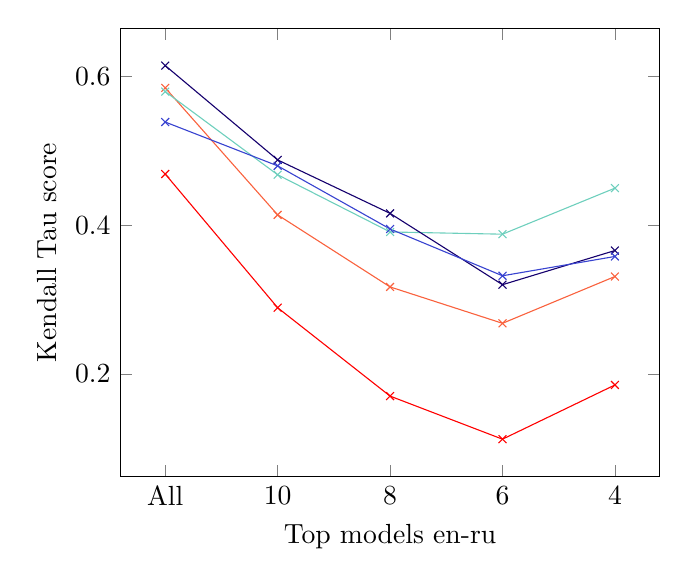
\begin{tikzpicture}
        \begin{axis}[
            xlabel=Top models en-ru, 
            ylabel=Kendall Tau score,
            xticklabels={ , , All, 10 , 8, 6, 4}
        ]
        
        \addplot[color=red,mark=x] coordinates {
        	(1, 0.469)
        	(2,  0.289)
        	(3,  0.170)
        	(4, 0.112)
        	(5 ,0.185)
        };
        
        \addplot[color=Unbabel5,mark=x] coordinates {
        	(1,  0.585)
        	(2, 0.414)
        	(3, 0.317)
        	(4, 0.268)
        	(5 , 0.331)
        };
        
        \addplot[color=Unbabel7,mark=x] coordinates {
        	(1,  0.580)
        	(2,  0.468)
        	(3,  0.391)
        	(4, 0.388)
        	(5 , 0.450)
        };
        
        \addplot[color=Unbabel2,mark=x] coordinates {
        	(1,  0.615)
        	(2,  0.488)
        	(3,  0.416)
        	(4, 0.320)
        	(5 , 0.366)
        };
        
        \addplot[color=Unbabel1,mark=x] coordinates {
        	(1,  0.539)
        	(2,  0.480)
        	(3,  0.395)
        	(4, 0.332)
        	(5 ,0.358)
        };
        \end{axis}
    \end{tikzpicture}
    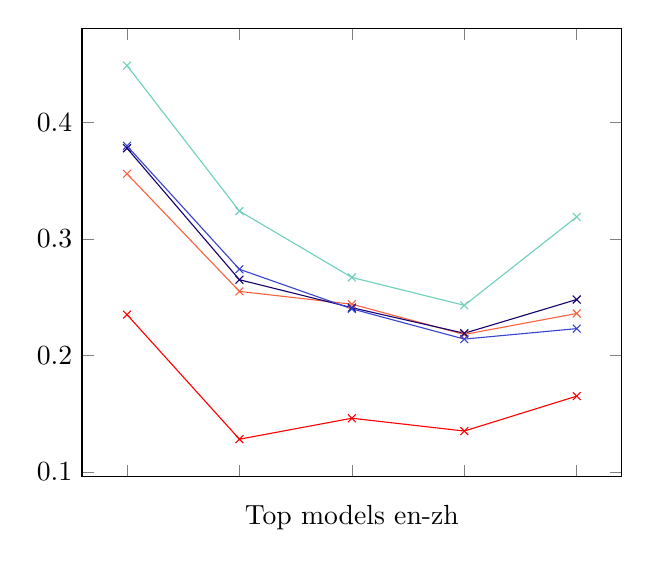
\begin{tikzpicture}
        \begin{axis}[
            xlabel=Top models en-zh, 
            xticklabels={ , , All, 10 , 8, 6, 4}
            legend style={font=\tiny},legend columns=2]
        ]
        	
        \addplot[color=red,mark=x] coordinates {
        	(1, 0.235)
        	(2, 0.128)
        	(3,  0.146)
        	(4, 0.135)
        	(5 ,0.165)
        };
        
        \addplot[color=Unbabel5,mark=x] coordinates {
        	(1,  0.356)
        	(2, 0.255)
        	(3, 0.244)
        	(4, 0.218)
        	(5 , 0.236)
        };
        
        \addplot[color=Unbabel7,mark=x] coordinates {
        	(1,  0.449)
        	(2,  0.324)
        	(3,  0.267)
        	(4, 0.243)
        	(5 , 0.319)
        };
        
        \addplot[color=Unbabel2,mark=x] coordinates {
        	(1,  0.378)
        	(2,  0.265)
        	(3,  0.241)
        	(4, 0.219)
        	(5 , 0.248)
        };
        
        \addplot[color=Unbabel1,mark=x] coordinates {
        	(1,  0.380)
        	(2,  0.274)
        	(3,  0.240)
        	(4, 0.214)
        	(5 ,0.223)
        };
        \end{axis}
        
    \end{tikzpicture}
\caption{Metrics performance over all and the top (10,8, 6, and 4) MT systems for all from-English language pairs. The color scheme is as follows: {\hwplotE} {\sc Comet-rank}, {\hwplotB} {\sc Comet-hter}, {\hwplotC} {\sc Comet-mqm}, {\hwplotA} {\sc Bleu}, {\hwplotF} {\sc Bertscore}}
\end{table*}%

\pgfplotsset{
	small,
}
\begin{table*}
\centering
    \begin{tabular}{ c c } 
	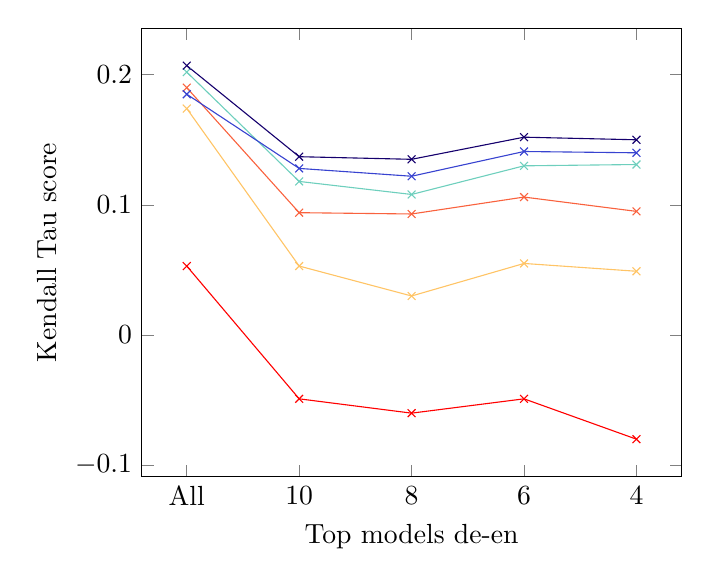
\begin{tikzpicture}
        \begin{axis}[
            xlabel=Top models de-en, 
            ylabel=Kendall Tau score,
            xticklabels={ , , All, 10 , 8, 6, 4}
        ]
        
        \addplot[color=red,mark=x] coordinates {
        	(1, 0.053)
        	(2,  -0.049)
        	(3,  -0.06)
        	(4, -0.049)
        	(5 ,-0.080)
        };
        
        \addplot[color=Unbabel5,mark=x] coordinates {
        	(1,  0.190)
        	(2,  0.094)
        	(3,  0.093)
        	(4, 0.106)
        	(5 , 0.095)
        };
        
        \addplot[color=Unbabel7,mark=x] coordinates {
        	(1,  0.202)
        	(2,  0.118)
        	(3,  0.108)
        	(4, 0.130)
        	(5 , 0.131)
        };
        
        
        \addplot[color=Unbabel2,mark=x] coordinates {
        	(1,  0.207)
        	(2,  0.137)
        	(3,  0.135)
        	(4, 0.152)
        	(5 , 0.150)
        };
         
        
        \addplot[color=Unbabel1,mark=x] coordinates {
        	(1,  0.185)
        	(2,  0.128)
        	(3,  0.122)
        	(4, 0.141)
        	(5 , 0.140)
        };
        
        \addplot[color=Unbabel4,mark=x] coordinates {
        	(1, 0.174)
        	(2,  0.053)
        	(3,  0.030)
        	(4, 0.055)
        	(5 , 0.049])
        };
	    \end{axis}
	\end{tikzpicture} &
	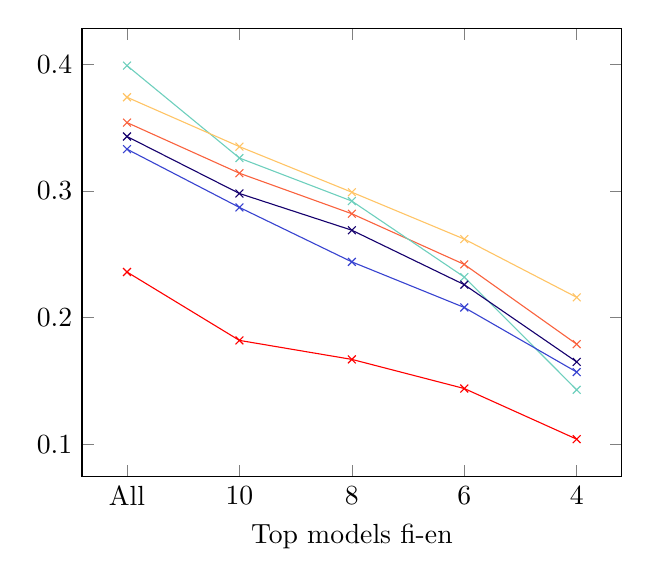
\begin{tikzpicture}
	    \begin{axis}[
            xlabel=Top models fi-en, 
            xticklabels={ , , All, 10 , 8, 6, 4}
        ]
        	
        \addplot[color=red,mark=x] coordinates {
        	(1, 0.236)
        	(2,  0.182)
        	(3,  0.167)
        	(4, 0.144)
        	(5 , 0.104)
        };
        
        \addplot[color=Unbabel5,mark=x] coordinates {
        	(1,  0.354)
        	(2,  0.314)
        	(3,  0.282)
        	(4, 0.242)
        	(5 , 0.179)
        };
        
        \addplot[color=Unbabel7,mark=x] coordinates {
        	(1,  0.399)
        	(2,  0.326)
        	(3,  0.292)
        	(4, 0.232)
        	(5 , 0.143)
        };
         
        \addplot[color=Unbabel2,mark=x] coordinates {
        	(1,  0.343)
        	(2,  0.298)
        	(3,  0.269)
        	(4, 0.226)
        	(5 , 0.165)
        };
         
        
        \addplot[color=Unbabel1,mark=x] coordinates {
        	(1,  0.333)
        	(2,  0.287)
        	(3,  0.244)
        	(4, 0.208)
        	(5 , 0.157)
        };
        
        \addplot[color=Unbabel4,mark=x] coordinates {
        	(1, 0.374)
        	(2,  0.335)
        	(3,  0.299)
        	(4, 0.262)
        	(5 , 0.216])
        };
        \end{axis}
    \end{tikzpicture} \\
    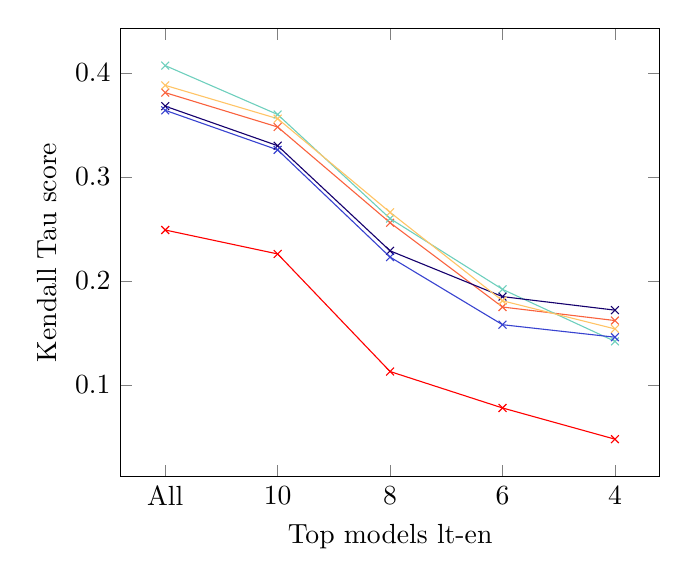
\begin{tikzpicture}
        \begin{axis}[
            xlabel=Top models lt-en, 
            ylabel=Kendall Tau score,
            xticklabels={ , , All, 10 , 8, 6, 4}
        ]
        	
        \addplot[color=red,mark=x] coordinates {
        	(1,0.249)
        	(2, 0.226)
        	(3, 0.1130)
        	(4, .078)
        	(5 ,0.048)
        };
        
        \addplot[color=Unbabel5,mark=x] coordinates {
        	(1,  0.381)
        	(2, 0.348)
        	(3,  0.256)
        	(4, 0.175)
        	(5 , 0.162)
        };
        
        \addplot[color=Unbabel7,mark=x] coordinates {
        	(1,  0.407)
        	(2,  0.360)
        	(3,  0.260)
        	(4, 0.192)
        	(5 , 0.142)
        };
        \addplot[color=Unbabel2,mark=x] coordinates {
        	(1,  0.368)
        	(2,  0.330)
        	(3,  0.229)
        	(4, 0.185)
        	(5 , 0.172)
        };
        \addplot[color=Unbabel1,mark=x] coordinates {
        	(1,  0.364)
        	(2,  0.326)
        	(3,  0.223)
        	(4, 0.158)
        	(5 , 0.146)
        };
        
        \addplot[color=Unbabel4,mark=x] coordinates {
        	(1, 0.388)
        	(2,  0.356)
        	(3,  0.266)
        	(4, 0.181)
        	(5 , 0.154])
        };
        \end{axis}
    \end{tikzpicture} &
    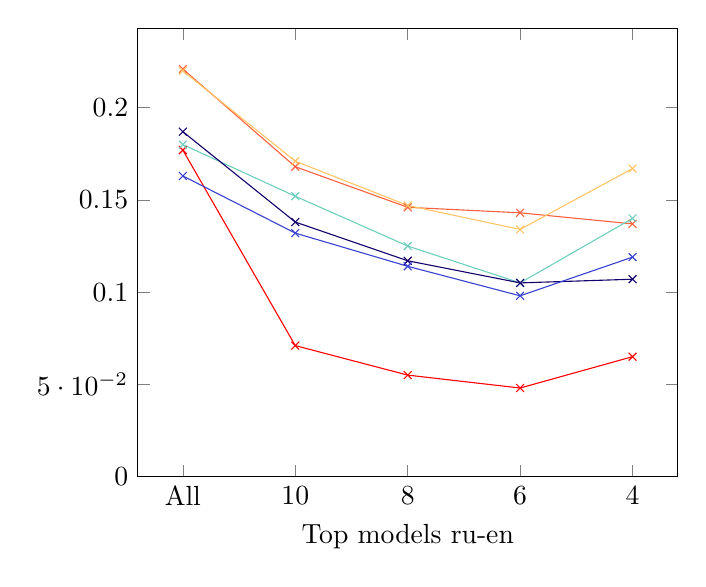
\begin{tikzpicture}
        \begin{axis}[
            xlabel=Top models ru-en, 
            xticklabels={ , , All, 10 , 8, 6, 4},
            ymin=0
        ]
        
        \addplot[color=red,mark=x] coordinates {
        	(1, 0.177)
        	(2,  0.071)
        	(3, 0.055)
        	(4, 0.048)
        	(5 , 0.065)
        };
        
        \addplot[color=Unbabel5,mark=x] coordinates {
        	(1,  0.221)
        	(2,  0.168)
        	(3,  0.146)
        	(4, 0.143)
        	(5 , 0.137)
        };
        
        \addplot[color=Unbabel7,mark=x] coordinates {
        	(1,  0.180)
        	(2,  0.152)
        	(3,  0.125)
        	(4, 0.105)
        	(5 ,0.140)
        };
         
        \addplot[color=Unbabel2,mark=x] coordinates {
        	(1,  0.187)
        	(2,  0.138)
        	(3,  0.117)
        	(4, 0.105)
        	(5 , 0.107)
        };
         
        \addplot[color=Unbabel1,mark=x] coordinates {
        	(1,  0.163)
        	(2,  0.132)
        	(3,  0.114)
        	(4, 0.098)
        	(5 , 0.119)
        };
        
        \addplot[color=Unbabel4,mark=x] coordinates {
        	(1, 0.220)
        	(2,  0.171)
        	(3,  0.147)
        	(4, 0.134)
        	(5 , 0.167])
        };
        \end{axis}
    \end{tikzpicture}
    \\
    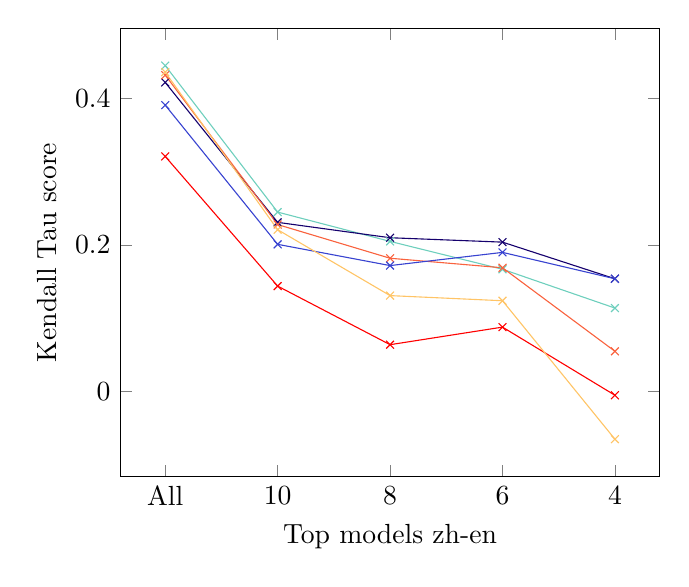
\begin{tikzpicture}
        \begin{axis}[
        	xlabel=Top models zh-en,
        	ylabel=Kendall Tau score,
        	xticklabels={ , , All, 10 , 8, 6, 4},
        ]

        \addplot[color=Unbabel7,mark=x] coordinates {
        	(1,  0.445)
        	(2,  0.245)
        	(3,  0.205)
        	(4, 0.167)
        	(5 , 0.114)
        };
        	
        \addplot[color=red,mark=x] coordinates {
        	(1,0.321)
        	(2, 0.144)
        	(3, 0.064)
        	(4,0.088)
        	(5 ,-0.005)
        };
        \addplot[color=Unbabel2,mark=x] coordinates {
        	(1,  0.422)
        	(2,  0.231)
        	(3,  0.210)
        	(4, 0.204)
        	(5 , 0.154)
        };
        
        \addplot[color=Unbabel5,mark=x] coordinates {
        	(1,  0.432)
        	(2, 0.228)
        	(3,  0.182)
        	(4, 0.169)
        	(5 , 0.055)
        };
        
        \addplot[color=Unbabel1,mark=x] coordinates {
        	(1,  0.391)
        	(2,  0.201)
        	(3,  0.172)
        	(4, 0.190)
        	(5 , 0.154)
        };
        
        \addplot[color=Unbabel4,mark=x] coordinates {
        	(1, 0.436)
        	(2,  0.221)
        	(3,  0.131)
        	(4, 0.124)
        	(5 ,-0.065])
        };
        \end{axis}
    \end{tikzpicture}
    \end{tabular}
\caption{Metrics performance over all and the top (10,8, 6, and 4) MT systems for all into-English language pairs. The color scheme is as follows: {\hwplotE} {\sc Comet-rank}, {\hwplotB} {\sc Comet-hter}, {\hwplotC} {\sc Comet-mqm}, {\hwplotA} {\sc Bleu}, {\hwplotF} {\sc Bertscore} , {\hwplotD} {\sc Bleurt}}
\end{table*}%

\end{document}
